\documentclass[main.tex]{subfiles}
\begin{document}
\chapter{Number Theory}

\epigraph{Time to get number \textit{freaky}.}{Justin Goodman}

\begin{center}
	\textit{This chapter is hefty.}
\end{center}

\minitoc

\section{Introduction}

\begin{defn}[Number Theory]
	The mathematical study of integers and their properties
\end{defn}

This chapter is intended to introduce you to the most important tool in number theory -- proofs. We will further explain how to execute a proof, however we must begin with basic definitions. It is important to see what is involved in a proof, so we will show you some proofs while introducing the basic principles.

\section{Basic Principles}

\subsection{Summations and Products}

We first introduce a form of notation that helps us simplify and express long equations.

\begin{defn}[Summation\index{Summation}]
	The sum over a sequence of numbers. Example: \[\sum_{\substack{i = 0 \\ i \text{ even}}}^{3} \frac{i+2}{i+1} = \frac{0+2}{0+1}+\frac{2+2}{2+1}+\frac{4+2}{4+1}+\frac{6+2}{6+1}\]
	
	Sometimes there is a condition (placed under the sum), which means you only evaluate the summation when the condition is \textit{satisfied}. Example: \[\sum_{\substack{i = 0 \\ i \text{ even}}}^{6} \frac{i+2}{i+1} = \frac{0+2}{0+1}+\frac{2+2}{2+1}+\frac{4+2}{4+1}+\frac{6+2}{6+1}\]
\end{defn}

The empty sum sums to zero and is denoted, for \(a > b\): \[\sum_{i = a}^{b} a_i = 0\]

\begin{defn}[Product\index{Product}]
	The product over a sequence of numbers. Example: \[\]
	
	Again, sometimes there is a condition (placed under the product), the same rules apply. Example: \[\prod_{\substack{i = 1 \\ i \text{ odd}}}^{8} i^2 = 1^2 \times 3^2 \times 5^2 \times 7^2\]
\end{defn}

The empty product multiplies to 1 and is denoted, for \(a > b\): \[\prod_{i = a}^{b} a_i = 1\]

\begin{rem}
	We can think of the indices in a sum or product as being elements of a set. Since the \(+\) operator is commutative, then the order that we evaluate the sum with respect to the indices \textit{does not matter}. For example, the sum \(\sum_{i=2}^{6} i\) iterates over the indices \(i \in \{2,3,4,5,6\}\), and equals \(2+3+4+5+6\) which can be re-ordered however we like (eg \(4+5+2+3+6\)). The condition placed on a sum or product simply becomes a restriction on the set. For example, the sum \(\sum_{\substack{i=2 \\ i \equiv 0 \Mod{3}}}^{6} i\) iterates over the indices \(\{i \in \{2,3,4,5,6\} \mid i \equiv 0 \Mod{3}\}\).
	
	Abstractly, we can write the sum (and similarly, the product) as a sum over elements of a set. We write this as follows: \[\sum_{\substack{i=a \\ P(i)}}^{b} a_i = \sum_{i \in I} a_i\] where \[I = \{i \in \Z \mid (a \leq i \leq b) \land P(i)\}\] and \(P(i)\) is the condition placed on the sum (or product).
	
	Interestingly, the condition placed on the summation (or product) can depend on the actual \textit{values} in the sum (or product). We could represent this as \(P(i) \equiv Q(a_i)\).
	
	Another interesting point, if we ever have \(a > b\) then the condition \(a \leq i \leq b\) is never satisfied, which means \(I = \emptyset\). We also have that if \(P(i)\) is false for all values of \(i\) such that \(a \leq i \leq b\), then again \(I = \emptyset\). If this is the case, then we sum (or product) over no indices. This is where the term \textbf{empty sum (or product)} comes from.
	
	The empty sum is equal to the additive identity 0, and the empty product is equal to the multiplicative identity 1 (as we have seen before).
\end{rem}

\exsol{
	Re-write the following sum as a summation, then evaluate it for \(n = 2\): \[\frac{1}{1} + \frac{2}{2} + \frac{3}{4} + \frac{4}{8} + \frac{5}{16} + \cdots + \frac{n+1}{2^n}\]
}{
	The sum equals \[\sum_{i = 0}^{n} \frac{i+1}{2^i}\] and for \(n=2\) evaluates to \[\frac{1}{1} + \frac{2}{2} + \frac{3}{4} = 2.75\]
}

\begin{defn}[Factorial\index{Factorial}]
	The factorial is the product, denoted \(n!\) for \(n \in \Z^+\), \[n! = \prod_{i=1}^{n} i\]
\end{defn}

\subsection{Sequences and Series}

We discuss sequences and series in a later chapter, however for now we introduce the basic ideas.

\begin{defn}[Sequence\index{Sequence}]
	An ordered list of numbers, each one associated with a specific \textit{position} (index)
\end{defn}

\begin{example}
	The following is a sequence: \[1,2,3,4,5,6,\cdots\]
	
	We can also write this surrounded by curly braces: \[\{1,2,3,4,5,6,\cdots\}\]
	
	We can also give this sequence as a function, which takes indices as the input: \[f(i) = i\]
	
	We can also denote the sequence with a name: \[a_i = i\]
\end{example}

\begin{defn}[Series\index{Series}]
	The sum of all terms in a sequence. Typically a series is infinite, however it can be finite.
\end{defn}

\begin{example}
	Let the sequence \(a_i = 2i\). Then we denote the infinite series: \[\sum_{i=1}^{\infty} a_i\]
	
	Methods from calculus can help us evaluate and understand infinite series, however that is out of scope of this course.
	
	If we give an upper bound, like \(n = 4\), then we can denote and evaluate finite series (which just becomes a summation): \[\sum_{i=1}^{4} a_i = 2(1) + 2(2) + 2(3) + 2(4) = 20\]
\end{example}

\subsection{Logarithms}

\begin{defn}[Exponentiation\index{Exponentiation}]
	The act of raising a fixed number \(n\) to a \textit{power} \(x\). You may be familiar with exponentiation with \(n,x \in \Q\) (for example, \(0.25^{0.5} = \frac{1}{\sqrt{4}} = 0.5\)), but in-fact we can define exponentiation on real inputs.
	
	Denote \(\exp x = \lim_{n \Rightarrow \infty} (1 + \frac{x}{n})^n = e^x\) with \(e^0 = 1\) and \(e^1 = e\). After defining logarithms below, we see that \(b = e^{\log b}\) so \(b^x = (e^{\log b})^x = e^{x \log b}\) which fully defines exponentiation.
\end{defn}

\(e = \sum_{n=0}^{\infty} \frac{1}{n!}\), \(e = \lim_{n \rightarrow \infty} (1 + \frac{1}{n})^n\), and \(e^x\) is the unique solution to the differential equation \(f(x) = f'(x)\) with \(f(0) = 1\).

\begin{defn}[Logarithm\index{Logarithm}]
	The function \(\log x\) is the inverse function of the exponential function \(e^x\). The logarithm satisfies \(\log 1 = 0\) and \(\log e = 1\). You may know this as the \textit{natural logarithm} \(\ln x = \log_e x\). If no base is given, assume the base is Euler's Number \(e\).
\end{defn}

Denote the \textit{base} \(b\) of a logarithm as \[\log_b x = \frac{\log x}{\log b}\]

\begin{prop}
	\[\log_b x + \log_b y = \log_b (x \cdot y)\]
\end{prop}

\begin{prop}
	\[a\log_b x = \log_b (x^a)\]
\end{prop}

\begin{prop}
	\[\log_b x - \log_b y = \log_b (xy^{-1}) = \log_b (\frac{x}{y})\]
\end{prop}

\begin{prop}
	\[a^{\log_b x} = x^{\log_b a}\]
\end{prop}

\subsection{Floors and Ceilings}

\begin{defn}[Floor\index{Floor}]
	The greatest integer less than or equal to the input real number. For \(x \in \R\), we denote the floor of \(x\) as \(\floor{x} = m \in \Z\) where \(m \leq x\) and \(m+1 > x\). So \[\floor{x} \leq x < \floor{x} + 1\]
	Equivalently, \[0 \leq x - \floor{x} < 1\] which means we can write \(x = \floor{x} + \epsilon\) with some \(\epsilon \in [0,1)\).
\end{defn}

\begin{defn}
	The smallest integer greater than or equal to the input real number. For \(x \in \R\), we denote the ceiling of \(x\) as \(\ceil{x} = n \in \Z\) where \(n \geq x\) and \(n-1 < x\). So \[\ceil{x} - 1 < x \leq \ceil{x}\]
	Equivalently, \[- 1 < x - \ceil{x} \leq 0\] which means we can write \(x = \ceil{x} + \epsilon\) with some \(\epsilon \in (-1,0]\). By negating \(\epsilon\), then \(x = \ceil{x} - \epsilon\) with some \(\epsilon \in [0,1)\).
\end{defn}

\exproof{
	Show that \(\floor{x+n} = \floor{x} + n\) for all \(x \in \R\) and \(n \in \Z\).
}{
	We can use any definition of the floor to prove this. The easiest proof comes from the second form.
	
	Denote \(\floor{x} = m \in \Z\). Then \(\floor{x} + n = m + n\) and \(\floor{x+n} = \floor{m + \epsilon + n} = \floor{m+n + \epsilon]} = m+n\) since \(m+n \in \Z\) by closure of integers under addition (this is discussed below).
}

\begin{rem}
	Similarly, \(\ceil{x+n} = \ceil{x} + n\).
\end{rem}

As a closing note, we should consider an interesting example in real analysis that uses floors to break intuition.

\exsol{
	\(\floor{0.9} = 0\), \(\floor{0.99} = 0\), \(\floor{0.999} = 0\), \(\floor{0.999\cdots9} = 0\). So what about \(\floor{0.\bar{9}}\)?
}{
	Intuitively, you might think that \(0.\bar{9} < 1\) which would mean \(\floor{0.\bar{9}} = 0\). This is incorrect, because by definition \(0.\bar{9} = 1\). This comes from how we define the bar operator, which means an infinite repetition of whatever is under it.
	\begin{align*}
		0.\bar{9} &= 0.9 + 0.09 + 0.009 + 0.0009 + \cdots \\
		&= 9(0.1 + 0.01 + 0.001 + 0.0001 + \cdots) \\
		&= 9(\frac{1}{10} + \frac{1}{100} + \frac{1}{1000} + \frac{1}{10000} + \cdots) \\
		&= 9\sum_{k=1}^{\infty} (\frac{1}{10})^k \\
		&= 9 \lim\limits_{n \rightarrow \infty} \sum_{k=1}^{n} (\frac{1}{10})^k \\
		&= 9 \lim\limits_{n \rightarrow \infty} [\sum_{k=0}^{n} (\frac{1}{10})^k - 1] \\
		&= 9 \lim\limits_{n \rightarrow \infty} [\frac{1 - (\frac{1}{10})^{n+1}}{1 - \frac{1}{10}} - 1] \\
		&= 9 \lim\limits_{n \rightarrow \infty} [\frac{10}{9}(1 - (\frac{1}{10})^{n+1}) - 1] \\
		&= 9 \lim\limits_{n \rightarrow \infty} [\frac{10}{9} - \frac{10}{9}(\frac{1}{10})^{n+1} - 1] \\
		&= 9 [ \frac{10}{9} - \frac{9}{9} - \frac{10}{9}\frac{1}{10} \lim\limits_{n \rightarrow \infty} (\frac{1}{10})^{n} ] \\
		&= 1 - \lim\limits_{n \rightarrow \infty} \frac{1}{10^n} = 1 - 0 = 1 \\
	\end{align*}
	Another way to see this, \[0.\bar{9} = 9 \cdot 0.\bar{1} = 9 \cdot \frac{1}{9} = 1\]
	
	Thus \[\floor{0.\bar{9}} = \floor{1} = 1\]
}

\begin{rem}
	This example uses a definition from real analysis. This book is on discrete mathematics. You do not need to know the definition of \(0.\bar{x}\)
\end{rem}

\subsection{Closure}

Closure has two parts: a \textbf{set}, and an \textbf{operation}. Closure is a \textit{property} of a set paired with the given operation. The basic idea is that if you take \textbf{any} two elements (or however are required for the operation -- typically two) and apply the given operation to those elements, then the result will be an element also in the set. Some examples will be helpful to illustrate the point here.

\begin{defn}[Closure\index{Closure}]
	For a given set \(S\) and operation \(\circ\), \(S\) is \textit{closed under} \(\circ\) if and only if \[(\forall a,b \in S)[a \circ b \in S]\]
	
	Note, the given operator could be unary, binary, trinary, etc, and the amount of variables pulled from the set correspond accordingly.
\end{defn}

\begin{thm}
	The natural numbers \(\N\) are closed under addition. Formally, \[(\forall n,m \in \N)[n+m \in \N]\]
\end{thm}

\begin{example}
	Try and think of some natural numbers where if you add them you \textit{do not} get a natural number. If you came up with an answer, it would be a \textit{counterexample} to the theorem.
	
	You should not be able to come up with a counterexample.
\end{example}

\begin{rem}
	For this book, we will accept the above theorem as a fact, since the proof relies on proposition \ref{ind-defn-N} (the inductive definition of \(\N\)) which we are not requiring you to know. The proof is relatively straightforward though, so we include it in a few sections.
\end{rem}

Okay, onto more examples of closure.

\exproof{
	The natural numbers are closed under multiplication. Formally, \[(\forall n,m \in \N)[n \cdot m \in \N]\]
}{
	Informal sketch: since \(m\) is a discrete counting number, we can think of \(n \cdot m = \underbrace{n + \cdots + n}_{m \text{ times}}\). Since \(\N\) is closed under addition, and multiplication here is just repeated addition, we are done.
}

\exproof{
	The natural numbers are \textbf{not} closed under subtraction. Formally, \[(\exists n,m \in \N)[n - m \not\in \N]\]
}{
	Take any natural numbers \(n,m\) such that \(n < m\). Then \(n < m \Rightarrow n - m < 0\) and we get a negative number, which is by definition not a natural number.
}

\begin{rem}
	This is somewhat rigorous. All we need here is a counterexample to \((\forall n,m \in \N)[n - m \in \N]\). So, just take any numbers that disprove the statement: \(5 - 6 = -1 \not\in \N\), done!
\end{rem}

\begin{thm}
	\[(\forall a,b \in \Z)[a + b \in \Z]\]
\end{thm}

\begin{rem}
	For the scope of this book, we can take it by definition that integers are closed under addition (the previous theorem).
\end{rem}

\exproof{
	Prove or disprove \[(\forall a,b \in \Z)[a \div b \in \Z]\]
}{
	Consider \(1,4 \in \Z\) but \(1 \div 4 = 0.25 \not\in \Z\), thus we have dis-proven the statement.
}

\exproof{
	Let \(S = \{1,2,3,4\}\). Show that \(S\) is not closed under addition.
}{
	Well, \(3,4 \in S\) but \(3+4 = 7 \not\in S\). Another counterexample: \(4+4 = 8 \not\in S\) (this is just to illustrate that you can pull \textbf{the same element} from the set since closure applies to \textbf{all} elements).
}

Closure can be of \textbf{any} set and \textbf{any} operation. We can get fancy with this, as with the previous example and the next example.

\exproof{
	Let \(S = \{a,b,c,d\}\). Define the following table as the outcome of performing a \(\blacklozenge\) operation:
	
	\begin{center}
		\begin{tabular}{c|cccc}
			& \(a\) & \(b\) & \(c\) & \(d\) \\
			\midrule
			\(a\) & \(d\) & \(c\) & \(b\) & \(a\) \\
			\(b\) & \(b\) & \(d\) & \(a\) & \(c\) \\
			\(c\) & \(c\) & \(a\) & \(d\) & \(b\) \\
			\(d\) & \(a\) & \(b\) & \(c\) & \(d\)
		\end{tabular}
	\end{center}
	
	For example, \(a \blacklozenge d = a\) (the first operand comes from the row, and the second operand comes from the column).
	
	Is \(S\) closed under \(\blacklozenge\)? Justify.
}{
	\(S\) is closed under \(\blacklozenge\) since every possible outcome (as listed in the table) of the \(\blacklozenge\) operation results in an element in \(S\).
}

Finally, we present an example of a unary operator.

\exproof{
	Show that the integers are closed under taking the negative (multiplying by \(-1\)), \[(\forall x \in \Z)[-x \in \Z]\]
}{
	Consider that \(-1 \in \Z\) and integers are closed under multiplication.
}

\subsection{Parity}

We introduce the idea with the definition.

\begin{defn}[Parity\index{Parity}]
	An inherit property of the integers which says that \textit{every} integer is \textit{exclusively} either \textbf{even} or \textbf{odd} (note the \textit{exclusive or} -- an integer must be even or odd, however it cannot be both and it cannot be neither)
\end{defn}

This is an important property and will be useful for later proofs. Imagine you want to show some statement is true for \textit{all} integers. Sometimes it is easier to break the statement into two cases -- odd integers and even integers -- and prove both cases separately. If both cases turn out to be true, then you can use parity to conclude the original statement is true.

We will show this idea in later proofs, however we should first explain what is even and odd.

\begin{defn}[Even\index{Parity!Even}]
	An integer \(n\) is even if and only if \((\exists k \in \Z)[n = 2k]\)
\end{defn}

\begin{defn}[Odd\index{Parity!Odd}]
	An integer \(m\) is odd if and only if \((\exists l \in \Z)[m = 2l + 1]\)
\end{defn}

By \textit{parity}, we can reformat the definitions of even and odd to depend on each other. The following statement is true:

\begin{center}
	An integer is even if and only if it is \textbf{not} odd
\end{center}

Equivalently:

\begin{center}
	An integer is odd if and only if it is \textbf{not} even
\end{center}

These statements both require that you know one of the two definitions. If this was not true, then the statements would be circular and would be useless.

We will come back to these statements soon.

\subsection{Divisibility}

Previously we showed that the integers are \textbf{not} closed under division. However, some integers when divided output an integer, like \(3/1\) and \(4/2\). It thus might make sense for us to study division.

\begin{defn}[Divisibility\index{Modular Arithmetic!Divisibility}]
	The property that a number can be evenly divided (with no remainder). \(a\) is divisible by \(b\) if and only if \(a \div b \in \Z\). Note that \(a \div b = \frac{a}{b}\).
	
	We say that \(b\) \textbf{divides} \(a\) if and only if \(a\) \textbf{is divisible by} \(b\), and we note this as \(b \mid a\). We will always use this notation.
	
	\[b \mid a \Leftrightarrow \frac{a}{b} \in \Z \Leftrightarrow (\exists x \in \Z)[a = bx]\]
\end{defn}

\begin{rem}
	We like to think of \(b \mid a \Leftrightarrow \frac{a}{b}\) as a rotation counterclockwise: \[\circarrowleft{$b \mid a$} \mapsto \frac{a}{b}\]
\end{rem}

\begin{defn}[Remainder\index{Modular Arithmetic!Remainder}]
	An alternate way to represent (integer) division. When \(b \nmid a\) then \(\exists r \in \Z\) where \(0 < r < a\) is the \textit{remainder} and \(b \mid (a - r)\). Sometimes we write the division as \(qRr\) -- this is just the integer part of the division \(q = (a-r)/b\) appended with \(R\) appended with the remainder
\end{defn}

\begin{thm}
	For any \(a,b \in \Z^+\), if \(b \mid a\) then \(b \leq a\)
\end{thm}

\begin{proof}
	\(b \mid a\) so by definition \((\exists k \in \Z)[\frac{a}{b} = k]\). Since \(a,b > 0\) we conclude that \(k > 0\). Since \(\frac{a}{b} = k\) then \(a = bk\). Since \(b,k > 0\) we conclude that \(bk \geq b\) and thus \(a = bk \geq b \Rightarrow b \leq a\)
\end{proof}

These definitions are important, however soon we will see that they fit into a wider scope of number theory. First, some examples.

\exsol{
	Give all natural numbers that divide 6.
}{
	We solve this by checking numbers. We do not want to check \textbf{all} numbers, though. Fortunately, we only have to check natural numbers, and the previous theorem tells us we only have to check numbers \(\leq 6\). Thus, we only need to check \(0,1,2,3,4,5,6\).
	\begin{itemize}
		\item We cannot divide by 0
		\item 1 divides everything
		\item 6 is even so \(2 \mid 6\)
		\item \(\frac{6}{3} = 2 \in \N\) % todo -- nicefrac ?
		\item \(\frac{6}{4} = 1.5 \not\in \N\)
		\item \(\frac{6}{5} = 1.2 \not\in \N\)
		\item Any integer divides itself, so \(6 \mid 6\)
	\end{itemize}
	Thus \(1,2,3,6\) divide 6.
}

\exsol{
	Find the remainder of 10 divided by 4.
}{
	We can repeatedly take away 4 from 11 until we're left with \(r\) such that \(0 < r < 4\).
	
	\(11 - 4 = 7\)
	
	\(7 - 4 = 3\)
	
	We did this process 2 times, so \(\frac{11}{4} = 2R3\). Also notice that \(\frac{11 - 3}{4} = 8/4 = 2\)
}

%\begin{example}
%	Show that 
%\end{example}

\subsection{Modular Arithmetic}

Modular arithmetic gives us a unified way to think about division between integers. Recall our definition of a remainder -- this is essentially what a modulus is, but with an important difference. We show some notation first, then the definitions.

\[a \equiv b \Mod{m}\]

\(a,b,m\) are all integers here, with \(m > 0\). Notice that we use the \(\equiv\) symbol, which we have seen is used for \textit{logical equivalence}. We will come back to this.

You may have seen modular arithmetic previously in a programming lens. In this case, the previous notation may be translated to the following.

\[a \ \% \ m = b\]

Still \(a,b,m\) are all integers but here we must have \(b < m\). This is exactly taking the remainder.

Here is the subtle difference -- in modular arithmetic, \(b\) \textbf{is not necessarily} less than \(m\).

\begin{defn}[Congruence\index{Modular Arithmetic!Congruence}]
	Two integers \(a\) and \(b\) are congruent with respect to an integer \(m\) if and only if \[\frac{b - a}{m}\] is an integer. This may be re-written as \[\big(\exists k \in \Z\big)\bigg[\frac{b-a}{m} = k\bigg]\]
\end{defn}

\begin{defn}[Modulus\index{Modular Arithmetic!Modulus}]
	The divisor \(m\) in the congruence of two integers
\end{defn}

\exsol{
	Find an integer congruent to 5 with respect to 3.
}{
	We can take the remainder of \(5/3\), which is 2. We will verify that \(2 \equiv 5 \Mod{3}\). Notice that \[\frac{5-2}{3} = \frac{3}{3} = 1\] which is an integer. Also notice that the order of \(a\) and \(b\) does not matter: \[\frac{2-5}{3} = \frac{-3}{3} = -1\] which is still an integer
	
	The problem asked for \textit{an} integer, so maybe other integers satisfy the congruence. We need to find an integer \(b\) such that \(\frac{b-5}{3} \in \Z\). We choose some random integer, maybe \(8\), and set it equal to the previous fraction, and solve for \(b\). \[\frac{b-5}{3} = 8 \Leftrightarrow b-5 = 24 \Leftrightarrow b = 29\] so 29 is congruent to 5, which is also congruent to 2, mod 3
}

You may have noticed how two integers are \textit{congruent}, not equal. We save \textit{equality} for things that are actually equal. Clearly \(29 \neq 2 \neq 5\) yet all of these integers are \textit{congruent} mod 3. This motivates a further expansion on congruence.

\begin{defn}[Congruence Class\index{Modular Arithmetic!Congruence Class}]
	The set of all integers that are congruent to each other with respect to a given modulus \(m\). For a given integer \(a\), the congruence class of \(a\) modulo \(m\) is the set of all integer solutions to \(\frac{b-a}{m} \in \Z\)
\end{defn}

\exsol{
	Write the set of all integers congruent to 3 modulo 5.
}{
	We need all integer solutions to \(\frac{b - 3}{5}\), or equivalently \(b = 5k+3\) for any integer \(k\). This is the set \[\{b \in \Z \mid (\exists k \in \Z)[b = 5k+3]\}\] which, if we plug in values for \(k\), equals \[\{\cdots, -12, -7, -2, 3, 8, 13,\cdots\}\]
}

\begin{rem}
	The congruence class of \(a\) modulo \(m\) is the set of all integers \(b\) such that \(a \equiv b \Mod{m}\).
\end{rem}

Now that you understand what \textit{is} modular arithmetic, we now discuss the difference between \textit{equivalence} and \textit{congruence}. In logic, as you have seen before, an \textit{equivalence} between two statements means that the two statements output the same truth values for the same inputs (the statements are \textit{logically equivalent}). In modular arithmetic, however, a \textit{congruence} between two integers means they fall in the same \textit{congruence class} modulo some number. We overload the \(\equiv\) symbol with these two meanings. Think of the \(\equiv\) operator as a function that takes two arguments. In the \textit{equivalence} definition the arguments are logical statements, however in the \textit{congruence} definition the arguments are integers. Logical statements and integers will never overlap, so you should never be confused by our usage of the operator.

Recall that we can use integer parity to relate our definitions of even and odd. We will see now \textit{why} it works.

\begin{thm}
	If two numbers are in different modulo classes, then they cannot be the same number. Formally, \[(\forall a,b \in \Z)(\forall m \in \Z^+)[a \not\equiv b \Mod{m} \Rightarrow a \neq b]\]
\end{thm}

\begin{proof}
	This is directly the contrapositive of an intuitive fact: \(a = b \Rightarrow a \equiv b \Mod{m}\). Consider that \(a \equiv a \Mod{m}\) and since \(a = b\) then \(a \equiv b \Mod{m}\)
\end{proof}


\exproof{
	Show that an even number cannot be an odd number.
}{
	Take an even number \(2k\) and an odd number \(2l+1\) for some \(k,l \in \Z\). Now mod-2 those numbers: \(2k \equiv 0 \Mod{2}\) and \(2l+1 \equiv 1 \Mod{2}\). Clearly \(0 \neq 1\) and hence by the previous theorem \(2k \neq 2l+1\). Thus an even number cannot be an odd number
}

Finally, three important theorems.

\begin{thm}
	For all integers \(a,b,c,d,m\) with \(m > 0\), if \[a \equiv b \Mod{m}\] and \[c \equiv d \Mod{m}\] then \[a+c \equiv b+d \Mod{m}\]
\end{thm}

\begin{proof}
	\(a \equiv b \Mod{m} \Leftrightarrow (\exists k \in \Z)[a = b + mk]\), \(c \equiv d \Mod{m} \Leftrightarrow (\exists l \in \Z)[c = d + ml]\). Then, we can add these two equations to get \(a+c = b + mk + d + ml = b+d + m(k+l)\). By closure of integers under addition, \(k+l \in \Z\), therefore \(a+c \equiv b+d \Mod{m}\)
\end{proof}

\begin{thm}
	For all integers \(a,b,c,d,m\) with \(m > 0\), if \[a \equiv b \Mod{m}\] and \[c \equiv d \Mod{m}\] then \[ac \equiv bd \Mod{m}\]
\end{thm}

\begin{proof}
	\(a \equiv b \Mod{m} \Leftrightarrow (\exists k \in \Z)[a = b + mk]\), \(c \equiv d \Mod{m} \Leftrightarrow (\exists l \in \Z)[c = d + ml]\). Then, we can multiply these two equations to get \(ac = (b + mk)(d + ml) = bd + bml + dmk + m^2lk = bd + m(bl + dk + mlk)\). By closure of integers under addition and multiplication, \(bl + dk + mlk \in \Z\), therefore \(ac \equiv bd \Mod{m}\)
\end{proof}

\begin{thm}
	For all integers \(a,b,m,n\) with \(m > 0\) and \(n \geq 0\), if \[a \equiv b \Mod{m}\] then \[a^n \equiv b^n \Mod{m}\]
\end{thm}

\begin{proof}
	For \(n = 0\) we have \(a^0 = 1\) and \(b^0 = 1\) and clearly \(1 \equiv 1 \Mod{m}\). For \(n = 1\) we have as given that \(a \equiv b \Mod{m}\). Finally \(n > 1\) follows by repeatedly taking the previous theorem letting \(c = a\) and \(d = b\).
\end{proof}

\begin{rem}
	The above theorem is a one-way implication. We cannot go the reverse direction. For example, \(2^4 = 16 \equiv 1 = 1^4 \Mod{3}\) yet \(2 \not\equiv 1 \Mod{3}\)
\end{rem}

\begin{rem}
	In all of the above theorems, the modulo \(m\) is the same. That is, we cannot do the following: \(8 \equiv 2 \Mod{6}\) and \(7 \equiv 1 \Mod{2}\) therefore \(8+7 \equiv 2+1 \Mod{???}\)
\end{rem}

\subsection{Number Bases}
\label{diff-num-bases}

Our familiar decimal system is known as \textit{base-10}, since we have 10 possible digits spanning 0 to 9. We can represent base-10 numbers as an addition of numbers multiplied by the associated decimal position (the ones place, tens, hundreds, thousands, etc...).

\begin{example}
	\(123 = 1 \cdot 10^2 + 2 \cdot 10^1 + 3 \cdot 10^0\)
\end{example}

There are three other bases important to computer science: base-2, base-8, and base-16.

\begin{defn}[Binary (base-2)]
	Representing numbers with two digits, 0 and 1
\end{defn}

\begin{defn}[Octal (base-8)]
	Representing numbers with digits 0 to 7
\end{defn}

\begin{defn}[Hexadecimal (base-16)]
	Representing numbers with 16 digits. After the 9th digit, we move to letters A through F
\end{defn}

We implicitly denote any number as base-10. If we want to denote a number \(x\) as base-\(b\), then we write \(x_b\). For example, the base-10 number \(24_{10}\) equals the base-2 number \(11000_2\).

\subsubsection{Techniques for Translation}

We generally work in base-10, so we will start with going from base-10 to any arbitrary base. For an arbitrary number \(x\) in base-10, translating it into a number in base \(b\) entails taking the least positive integer of \(x\) modulo \(b\), integer dividing with respect to the base (by taking \(\floor{x/b}\), and repeating until the number becomes zero. This will yield a sequence of integers, which make up the digits of the number in base-\(b\) from least to most significant (right to left).

\exsol{
	Find the base-5 representation of the base-10 number 12345.
}{
	Follow the given algorithm. Step-wise, we get:
	
	\begin{enumerate}
		\item \(12345 \equiv 0 \Mod{5}\), and \(\floor{12345/5} = 2469\)
		\item \(2469 \equiv 4 \Mod{5}\), and \(\floor{2469/5} = 493\)
		\item \(493 \equiv 3 \Mod{5}\), and \(\floor{493/5} = 98\)
		\item \(98 \equiv 3 \Mod{5}\), and \(\floor{98/5} = 19\)
		\item \(19 \equiv 4 \Mod{5}\), and \(\floor{19/5} = 3\)
		\item \(3 \equiv 3 \Mod{5}\), and \(\floor{3/5} = 0\)
	\end{enumerate}
	So \(12345_{10} = 343340_5\)
}

We care more about the special cases of \(b\) here -- 2, 8, and 16. We start with base-2.

A binary number's digits represent powers of 2 in base-10. For example, \(18_{10} = 10010_2 = 16_{10} + 2_{10} = 1 \cdot 2^4 + 0 \cdot 2^3 + 0 \cdot 2^2 + 1 \cdot 2^1 + 0 \cdot 2^0\)
\begin{center}
	\begin{tabular}{cccccc}
		\(\cdots\) & 16 & 8 & 4 & 2 & 1 \\
		\midrule
		\(\cdots\) & 1 & 0 & 0 & 1 & 0 \\
	\end{tabular}
\end{center}

\begin{boxx}
	\textbf{Translating base-10 to base-2:} Associate each binary digit with a power of 2 -- \(\{1,2,4,8,16,32,\cdots\}\) -- then repeatedly, until the input number becomes zero, subtract the highest power of 2 lower than the input number. The powers of 2 subtracted get a 1 for their digit, and the others get a 0.
\end{boxx}

\exsol{
	Translate 43 to binary.
}{
	\\
	\begin{enumerate}
		\item The highest power of 2 lower than 43 is 32, so the 32 digit gets a 1. \(43-32 = 11\)
		\item The highest power of 2 lower than 11 is 8, so the 8 digit gets a 1. \(11-8=3\)
		\item The highest power of 2 lower than 3 is 2, so the 2 digit gets a 1. \(3-2=1\)
		\item The highest power of 2 lower than 1 is 1, so the 1 digit gets a 1. \(1-1=0\)
	\end{enumerate}
	So \(43_{10} = 101011_2\)
}

\begin{boxx}
	\textbf{Translating base-10 to base-16:} First, translate the number to binary. Append zeros to the left-side of the binary number until the number of digits is a multiple of 4. Next, partition the number into groups of four (4) digits (bits). Finally, translate each 4-digit binary number group into a hexadecimal digit 0-15 (0-\(F\)).
\end{boxx}

\exsol{
	Translate 43 to hexadecimal.
}{
	From before, \(43_{10} = 101011_2\). Left-fill with zeros: \(= 00101011_2\). Partition into groups of 4: \(= 0010 \mid 1011\). Translate each group into a hex number: \(0010_2 = 2_{10} = 2_{16}\) and \(1011_2 = 11_{10} = B_{16}\). So \(43_{10} = 2B_{16}\)
}

\begin{boxx}
	\textbf{Translating base-10 to base-8:} (\textit{similar to the previous method}) First, translate the number to binary. Append zeros to the left-side of the binary number until the number of digits is a multiple of 3. Next, partition the number into groups of three (3) digits (bits). Finally, translate each 3-digit binary number group into an octal digit 0-7.
\end{boxx}

\exsol{
	Translate 43 to octal.
}{
	From before, \(43_{10} = 101011_2\). Left-fill with zeros (none required): \(= 101011_2\). Partition into groups of 3: \(= 101 \mid 011\). Translate each group into an octal number: \(101_2 = 5_{10} = 5_8\) and \(011_2 = 3_{10} = 3_8\). So \(43_{10} = 53_8\)
}

\begin{rem}
	We need four (4) binary digits to represent numbers 0-15, and three (3) binary digits to represent numbers 0-7.
\end{rem}

Now, how do we go back from base-\(b\) to base-10? Well, associate each digit into an index position \(i\), then multiply that digit by the base \(b\) raised to the power \(i\).

\begin{example}
	\(2B_{16} = 2 \cdot 16^1 + B \cdot 16^0 = 2 \cdot 16 + 11 = 32 + 11 = 43\)
\end{example}

Finally, how do we arbitrarily translate between bases? Well, usually the fastest way is to translate to base-10 or base-2, then translate to the other base you need.

\subsubsection{Fast Mods}

Taking mods with certain modulo can be made very easy, so long as you understand the previous modular arithmetic theorems and base-10 expansion.

\begin{boxx}
	\textbf{Mod 1:} Just return 1, since everything is divisible by 1.
\end{boxx}

\begin{boxx}
	\textbf{Mod 2:} Return 0 if the integer is even, and 1 if the integer is odd.
\end{boxx}

\begin{boxx}
	\textbf{Mod 3:} Notice that \(10^k \equiv 1 \Mod{3}\) for all \(k \in \N\). So we expand an input number as the base-10 representation \(a_n \cdot 10^n + \cdots + a_2 \cdot 10^2 + a_1 \cdot 10^1 + a_0 \cdot 10^0\) where the \(a_i\)'s make up the associated digits of the input number. Then we take this summation \(\Mod{3}\) and we get \[a_n \cdot 10^n + \cdots + a_2 \cdot 10^2 + a_1 \cdot 10^1 + a_0 \cdot 10^0 \equiv a_n + \cdots + a_2 + a_1 + a_0 \Mod{3}\]
	
	Thus, any integer is congruent to the sum of its digits \(\Mod{3}\).
\end{boxx}

\begin{boxx}
	\textbf{Mod 5:} Notice that \(10^k \equiv 0 \Mod{5}\) for all \(k \in \N\) with \(k > 0\). So, any digit past the one's place is equivalent to 0 \(\Mod{5}\), \[a_n \cdot 10^n + \cdots + a_2 \cdot 10^2 + a_1 \cdot 10^1 + a_0 \cdot 10^0 \equiv 0a_n + \cdots + 0a_2 + 0a_1 + 1a_0 \equiv a_0 \Mod{5}\]
	
	Thus, any integer is congruent to its one's place digit \(\Mod{5}\).
\end{boxx}

\begin{boxx}
	\textbf{Mod 9:} Works exactly the same way as \(\Mod{3}\), since \(10^k \equiv 1 \Mod{9}\) for all \(k \in \N\).
\end{boxx}

\begin{boxx}
	\textbf{Mod 10:} Return the digit in the one's place (the last digit) of the input integer.
\end{boxx}

\subsubsection{Applications to Circuits}

One application which we promised to discuss is binary addition and its relation to circuits.

We can build a circuit that adds two single-digit binary numbers? There are only 4 possibilities for adding single-digit numbers, so let's examine what a truth table for this process might look like (all numbers are in base-2):
	
\begin{center}
	\begin{tabular}{cc|c}
		input \(a\) & input \(b\) & output \(a + b\) \\
		\midrule
		0 & 0 & 0 \\
		0 & 1 & 1 \\
		1 & 0 & 1 \\
		1 & 1 & 10 \\
	\end{tabular}
\end{center}

In the output, we can always append zeros to the beginning of the binary number without changing the actual number:

\begin{center}
	\begin{tabular}{cc|c}
		input \(a\) & input \(b\) & output \(a + b\) \\
		\midrule
		0 & 0 & 00 \\
		0 & 1 & 01 \\
		1 & 0 & 01 \\
		1 & 1 & 10 \\
	\end{tabular}
\end{center}

Now let's separate our output column into two columns -- the sum-bit (right) and the carry-bit (left):

\begin{center}
	\begin{tabular}{cc|cc}
		input \(a\) & input \(b\) & carry & sum \\
		\midrule
		0 & 0 & 0 & 0 \\
		0 & 1 & 0 & 1 \\
		1 & 0 & 0 & 1 \\
		1 & 1 & 1 & 0 \\
	\end{tabular}
\end{center}

We know how to generate Boolean expressions for the output columns: 
\begin{align*}
\text{sum} &\equiv a \oplus b \\
\text{carry} &\equiv a \land b
\end{align*}

Which gives us the \textbf{half adder}:

\begin{boxx}
	Adding two bits \(a+b = cs\) is equivalent to the circuit
	\begin{center}
		\begin{circuitikz}
			\draw
			(0,0) node (xor1) [xor port] {}
			(0,1.5) node (and1) [and port] {}
			(and1.in 1) node (a) [anchor=east,xshift=-1cm] {\(a\)}
			(xor1.in 2) node (b) [anchor=east,xshift=-1cm] {\(b\)};
			
			\draw (and1.in 1) -- (a);
			\draw (and1.in 2) -- (b);
			\draw (xor1.in 1) -- (a);
			\draw (xor1.in 2) -- (b);
			
			\draw
			(and1.out) node (c) [anchor=west,xshift=1cm] {carry}
			(xor1.out) node (s) [anchor=west,xshift=1cm] {sum};
			
			\draw (and1.out) -- (c);
			\draw (xor1.out) -- (s);
			
			\node [xshift=.2cm] at (a) {\textbullet};
			\node [xshift=.2cm] at (b) {\textbullet};
			\node [xshift=-.5cm] at (c) {\textbullet};
			\node [xshift=-.5cm] at (s) {\textbullet};
		\end{circuitikz}
	\end{center}
\end{boxx}

Now we can add two 1-bit numbers together. What if we want to add multiple-bit numbers together? Consider adding two 2-bit numbers:
\begin{center}
	\begin{tabular}{ccc}
		& \(c\) & \\
		& \(x\) & \(y\) \\
		\(+\) & \(z\) & \(w\) \\
		\midrule
		\(o_2\) & \(o_1\) & \(s\)
	\end{tabular}
\end{center}

We see here that after adding \(y+w\) we are left with a carry bit \(c\) for our addition \(x+z\). How do we add three bits \(c+x+z\)? Well, we can separate it into two 1-bit additions: \(c+x\) which, via a half-adder, yields a sum bit \(s_1\) and carry bit \(c_1\), then \(s_1 + z\) which, via another half-adder, yields a sum bit \(s_2\) and carry bit \(c_2\). Then, we can let \(o_1 = s_2\). Unfortunately this leaves us two carry bits that somehow need to be combined into a final carry bit.

Consider now the truth-table for adding three bits:
\begin{center}
	\begin{tabular}{ccc|c|ccc}
		\(c\) & \(x\) & \(z\) & \(c+x+z\) & carry\((c+x)\)  & sum\((c+x) = s_1\) & carry\((s_1+z)\) \\
		\midrule
		0 & 0 & 0 & 00 & 0 & 0 & 0 \\
		0 & 0 & 1 & 01 & 0 & 0 & 0 \\
		0 & 1 & 0 & 01 & 0 & 1 & 0 \\
		0 & 1 & 1 & 10 & 0 & 1 & 1 \\
		1 & 0 & 0 & 01 & 0 & 1 & 0 \\
		1 & 0 & 1 & 10 & 0 & 1 & 1 \\
		1 & 1 & 0 & 10 & 1 & 0 & 0 \\
		1 & 1 & 1 & 11 & 1 & 0 & 0 \\
	\end{tabular}
\end{center}

Now notice the carry bit in the output column \(c+x+z\) is the same as OR-ing the two carry bits from \(c+x\) and \(s_1+z\). This completes our circuit for adding three bits. We call this the \textbf{full adder}:

\begin{boxx}
	Adding three bits \(a+b+c = os\) is equivalent to the circuit
	\begin{center}
		\begin{circuitikz}
			\draw
			(0,0.75) node[draw,minimum width=2cm,minimum height=1cm] (HA1) {Half Adder}
			(3.5,0) node[draw,minimum width=2cm,minimum height=1cm] (HA2) {Half Adder}
			($(HA1.west)!0.75!(HA1.north west)$) coordinate (ha1in1)
			($(HA1.west)!0.75!(HA1.south west)$) coordinate (ha1in2);
			\draw
			(ha1in1) node (a) [anchor=east,xshift=-0.5cm] {\(a\)}
			(ha1in2) node (b) [anchor=east,xshift=-0.5cm] {\(b\)}
			(ha1in1) -- (a)
			(ha1in2) -- (b);
			\node [xshift=.2cm] at (a) {\textbullet};
			\node [xshift=.2cm] at (b) {\textbullet};
			
			\draw
			($(HA1.east)!0.75!(HA1.north east)$) coordinate (ha1out1)
			($(HA1.east)!0.75!(HA1.south east)$) coordinate (ha1out2);
			\draw
			(ha1out1) node (c1) [anchor=west,xshift=4cm] {c\(_1\)}
			(ha1out2) node (s1) [anchor=west,xshift=0.35cm] {sum}
			(ha1out1) -- (c1)
			(ha1out2) -- (s1);
			%\node [xshift=-.2cm] at (c1) {\textbullet};
			
			\draw
			($(HA2.west)!0.75!(HA2.north west)$) coordinate (ha2in1)
			($(HA2.west)!0.75!(HA2.south west)$) coordinate (ha2in2);
			\draw
			(s1) -- (ha2in1)
			(ha2in2) node (c) [anchor=east,xshift=-4cm] {\(c\)}
			(ha2in2) -- (c);
			\node [xshift=.2cm] at (c) {\textbullet};
			
			\draw
			($(HA2.east)!0.75!(HA2.north east)$) coordinate (ha2out1)
			($(HA2.east)!0.75!(HA2.south east)$) coordinate (ha2out2);
			\draw
			(ha2out1) node (c2) [anchor=west,xshift=0.5cm] {c\(_2\)}
			(ha2out2) node (s) [anchor=west,xshift=2.65cm] {\(s\)}
			(ha2out1) -- (c2)
			(ha2out2) -- (s);
			\node [xshift=-.2cm] at (s) {\textbullet};
			
			\draw
			(7,0.75) node (or1) [or port] {}
			(or1.in 1) -- (c1)
			(or1.in 2) -- (c2)
			(or1.out) node (o) [anchor=west] {\(o\)};
			\node [xshift=-.2cm] at (o) {\textbullet};
		\end{circuitikz}
	\end{center}
\end{boxx}

Putting these two structures, the half adder and full adder, together, we can construct a 2-bit adder, which solves our previous problem of doing \(xy + zw = o_2o_1s\):

\begin{boxx}
	Adding three bits \(a+b+c = os\) is equivalent to the circuit
	\begin{center}
		\begin{circuitikz}
			\draw
			(0,0.75) node[draw,minimum width=2cm,minimum height=1cm] (HA1) {Half Adder}
			(3.75,-0.2) node[draw,minimum width=2cm,minimum height=1.5cm] (FA1) {Full Adder}
			($(HA1.west)!0.75!(HA1.north west)$) coordinate (ha1in1)
			($(HA1.west)!0.75!(HA1.south west)$) coordinate (ha1in2);
			\draw
			(ha1in1) node (y) [anchor=east,xshift=-0.5cm] {\(y\)}
			(ha1in2) node (w) [anchor=east,xshift=-0.5cm] {\(w\)}
			(ha1in1) -- (y)
			(ha1in2) -- (w);
			\node [xshift=.2cm] at (y) {\textbullet};
			\node [xshift=.2cm] at (w) {\textbullet};
			
			\draw
			($(HA1.east)!0.75!(HA1.north east)$) coordinate (ha1out1)
			($(HA1.east)!0.75!(HA1.south east)$) coordinate (ha1out2);
			\draw
			(ha1out1) node (s) [anchor=west,xshift=4.5cm] {\(s\)}
			(ha1out2) node (c1) [anchor=west,xshift=0.35cm] {carry}
			(ha1out1) -- (s)
			(ha1out2) -- (c1);
			\node [xshift=-.2cm] at (s) {\textbullet};
			
			\draw
			($(FA1.west)!0.75!(FA1.north west)$) coordinate (fa1in1)
			($(FA1.west)!0.75!(FA1.south west)$) coordinate (fa1in2)
			($(FA1.west)!0!(FA1.south west)$) coordinate (fa1in3);
			\draw
			(c1) -- (fa1in1)
			(fa1in2) node (x) [anchor=east,xshift=-4.25cm] {\(x\)}
			(fa1in2) -- (x)
			(fa1in3) node (z) [anchor=east,xshift=-4.25cm] {\(z\)}
			(fa1in3) -- (z);
			\node [xshift=.2cm] at (x) {\textbullet};
			\node [xshift=.2cm] at (z) {\textbullet};
			
			\draw
			($(FA1.east)!0.75!(FA1.north east)$) coordinate (fa1out1)
			($(FA1.east)!0.75!(FA1.south east)$) coordinate (fa1out2);
			\draw
			(fa1out1) node (o1) [anchor=west,xshift=0.75cm] { \(o_1\)}
			(fa1out2) node (o2) [anchor=west,xshift=0.75cm] { \(o_2\)}
			(fa1out1) -- (o1)
			(fa1out2) -- (o2);
			\node [xshift=-.3cm] at (o1) {\textbullet};
			\node [xshift=-.3cm] at (o2) {\textbullet};
		\end{circuitikz}
	\end{center}
\end{boxx}

This solves our 2-bit addition problem. What if we want to add 3-bit numbers? 4-bit numbers? \(n\)-bit numbers? Well, after the first bit column (adding two bits) we must add three bits. After this second column, we get a sum bit and a carry bit. If we tack on another column, which would make a 3-bit adder, then we add in the previous carry to the two new bits. This same process repeats for all further columns. So, tacking on another bit solely entails tacking on another full adder! \textit{Picture omitted}.

\exsol{
	How many half adders are required for an \(n\)-bit adder?
}{
	Note, here we implicitly assumed \(n > 0\).
	
	We need 1 half adder to start, and we need \(n-1\) full adders which each contain 2 half adders. This totals to \(2(n-1) + 1 = 2n-1\) half adders.
}

\section{Proofs -- Introduction}

Recall that number theory studies integers \textit{and their properties}. We want to think about certain properties and be able to explain why they hold. We want our explanations, \textit{proofs}, to be valid. We want to take our knowledge base of basic principles and logically derive true/false statements. The whole idea behind a proof is to creatively apply the set of rules you know to show whether a statement hold or not.

\begin{defn}[Proof\index{Proof}]
	A formal and logical explanation for why a statement is true or false.
\end{defn}

Let's examine this definition. We want to explain why a statement is \textit{true} or \textit{false}. Recall that in first-order logic (predicate logic) we have \textit{existential} statements and \textit{universal} statements. This gives us four proof ``bins'':

\begin{tabularx}{\textwidth}{lXX}
	\toprule
	& Proving True & Proving False \\
	\midrule
	Existential Statement & Find an example that makes the statement True & Show the statement is False for every element \\
	\midrule
	Universal Statement & Show the statement is True for every element & Find an example that makes the statement False \\
	\bottomrule
\end{tabularx}

Proving an existential statement true, as well as proving a universal statement false, is relatively easy -- all you must do is search the statement domain for an example. Comparatively, proving an existential statement false, as well as proving a universal statement true, is much harder since it takes some form of creativity -- that is, if you believe \(P \neq NP\)\footnote{You will learn about this in an Algorithms course. Here is the gist: problems in the \(N\)on-deterministic \(P\)olynomial (\(NP\)) class are ones whose solution is \textit{easy} to verify in Polynomial time. \(P\)olynomial class problems have Polynomial-time (relatively fast) algorithms. If \(P = NP\) then problems whose solution is easy to check \textit{also} have fast algorithms. Typically you must use creativity to come up with an algorithm, however if it is just as easy to check a solution as it is to come up with a solution generator (algorithm), then creativity becomes meaningless. \href{https://youtu.be/YX40hbAHx3s}{Suggested reading}.}.

Before we continue, we must show you how to format your proofs. The structure in this book may be different than what your instructor prefers, so make sure you pay attention in class and follow what they do. Our structure, however, is quite flexible with minimal rules, so it should be easy to adapt. You have likely already seen our style of proof in this book. We always follow a simple structural format that puts ``\textit{Proof.}'' at the start, followed by what technique we are using (typically), followed by our explanation, finished by a simple square signifying the end of the proof.

\begin{proof}
	\(\leftarrow\) this signifies the start of a proof
	
	\vspace{2em}
	
	\begin{center}
		\(\dots\) put logically-sound proof here \(\dots\)
	\end{center}
	
	\vspace{2em}
	
	\hfill \(\dots \dots \dots \dots \dots \dots \dots \dots \) and this signifies the end of a proof \(\rightarrow\)
\end{proof}

The ``\textit{Proof.}'' header clearly signifies the following text will be a proof and should be read as such.

The ending square is shorthand for the latin phrase \textit{quod erot demonstrandum} which, used in this context, roughly means \textit{it is shown/demonstrated}. You may put any of the following at the end of your proofs: QED, \(\blacksquare\), \(\square\).

This general structure is easy to read, easy to adapt, and is easily formal. It is \textit{absolutely fine} to deviate from our structure, \textbf{so long as} your proof is still easy to read and makes clear it \textbf{is} a proof.

\exproof{ % todo -- move somewhere else?
	Pythagoras' Theorem states that for any right-triangle, the square of the hypotenuse equals the sum of the squares of the other two sides. More familiarly, \[a^2 + b^2 = c^2\]
	Prove it.
}{
	Make 4 copies of a right triangle, and arrange them like so:
	\begin{center}
		\begin{tikzpicture}
		% outer square
		\draw (0,0) -- (5,0);
		\draw (0,0) -- (0,5);
		\draw (0,5) -- (5,5);
		\draw (5,0) -- (5,5);
		% inner square
		\draw (0,4) -- (4,5);
		\draw (4,5) -- (5,1);
		\draw (5,1) -- (1,0);
		\draw (1,0) -- (0,4);
		% letters
		\draw (-0.25,4.5) node {\(a\)};
		\draw (2,5.25) node {\(b\)};
		\draw (4.5,5.25) node {\(a\)};
		\draw (5.25,3) node {\(b\)};
		\draw (5.25,0.5) node {\(a\)};
		\draw (3,-0.25) node {\(b\)};
		\draw (0.5,-0.25) node {\(a\)};
		\draw (-0.25,2) node {\(b\)};
		\end{tikzpicture}
	\end{center}
	The area of the inner square is then \[(a+b)^2 - 4(\frac{1}{2}ab) = a^2 + 2ab + b^2 - 2ab = a^2 + b^2\]
	
	Denote the side length of each edge of the inner square \(c\) -- which is also the hypotenuse of each right-triangle. Then \(c^2\) is the area of the inner square, so \[c^2 = a^2 +  b^2\]
}

\begin{rem}
	We do not expect you to know how to prove Pythagoras' Theorem -- this is just an interesting proof example.
\end{rem}

\section{Proofs -- Techniques}

We have a handful of proof techniques that will help you structure your proofs.

\subsection{Direct Proof}

Direct proofs are classical applications of valid reasoning (see chapter \ref{section:reasoning} about deductions). We start with the easier techniques: examples and counter-examples.

\begin{defn}[Proof by Example]
	Showing a statement is true by presenting an example. This is used for proving existential statements true
\end{defn}

\exproof{
	Prove that there is an integer that divides 6.
}{
	\(\frac{6}{2} = 3 \in \Z\) so by definition \(2 \mid 6\), so 2 is an example.
}

\exproof{
	Show that \[(\exists z \in \Z)(\forall n \in \N)[z \leq n]\]
}{
	The naturals are all positive, so any negative integer works. Let \(z = -1 \leq n\) for all \(n \in \N\) be our example.
}

\begin{defn}[Proof by Counterexample]
	Showing a statement is false by presenting a counterexample. This is used for proving universal statements false
\end{defn}

\exproof{
	Prove false that all integers are divisible by 3.
}{
	\(3 \nmid 2\), so 2 is a counterexample.
}

\begin{rem}
	Proof by example and counterexample are the same. To see this, consider a general existential statement we want to prove true: \[(\exists x)[P(x)] \equiv t\]
	Now consider a general universal statement we want to prove false, and negate the entire thing: \[\lnot ((\forall x)[Q(x)] \equiv f)\] \[(\exists x)[\lnot Q(x)] \equiv t\]
	By letting \(Q(x) \equiv \lnot P(x)\) then we recover a proof by example.
\end{rem}

\begin{defn}[Proof by Exhaustion]
	Proving a statement by reasoning about every possibility. Typically used for statements about small sets
\end{defn}

\exproof{
	Prove that \((\forall e \in \{3,6,9\})[3 \mid e]\)
}{
	We proceed via proof by exhaustion.
	
	There are three possible cases in this statement: \(3 \mid 3\), \(3 \mid 6\), \(3 \mid 9\)
	
	Case 1: \(e = 3\), well \(3 \mid 3\) since \(\frac{3}{3} = 1 \in \Z\)
	
	Case 2: \(e = 6\), well \(3 \mid 6\) since \(\frac{6}{3} = 2 \in \Z\)
	
	Case 3: \(e = 9\), well \(3 \mid 9\) since \(\frac{9}{3} = 3 \in \Z\)
	
	All cases cover the domain, and all are true, therefore the statement is true.
}

\begin{defn}[Proof by Construction]
	Proving an existential statement by giving an algorithm or method to create the object in the statement.
\end{defn}

\exproof{
	Show that there exist irrational numbers \(a,b\) such that \(a^b\) is rational.
}{
	We will show this by constructing an actual example. First note that \(\sqrt{2}\) is irrational. We will prove this later. Next, note that \(\log_2(9)\) is irrational. We will also prove this later.
}

\exproof{
	Prove \textbf{false} that \((\forall n \in \Z)[n \equiv 1 \Mod{4}]\).
}{
	This is probably obvious, since \(m = 6 \in \Z\) has \(m \equiv 2 \not\equiv 1 \Mod{4}\).
	
	Consider another, constructive argument. We will construct a counterexample. So suppose \(n \equiv 1 \Mod{4}\), then \(\exists k \in \Z\) such that \(n = 1 + 4k\). Then \(2n = 2(1+4k) = 2+8k = 2+4(4k) \equiv 2 \not\equiv 1 \Mod{4}\). So to construct a counterexample, we can simply double our input number \(n\).
}

\begin{defn}[Proof by Non-Construction]
	Proving an existential statement \textit{without} providing an example, or a way to construct an example.
\end{defn}

The following is a classic non-constructive proof of the previous example (theorem).

\exproof{
	Show that exist irrational numbers \(a,b\) such that \(a^b\) is rational.
}{
	This time, we will do this without necessarily fixing some precise values for \(a\) and \(b\).
	
	Note again (we will prove later) that \(\sqrt{2}\) is irrational. Then consider the number \(\sqrt{2}^{\sqrt{2}}\). This number is either \textit{rational} or \textit{irrational} (there are no other options, since it is a real number).
	
	\textbf{If} \(\sqrt{2}^{\sqrt{2}}\) is \textit{rational}, then, since \(\sqrt{2}\) is irrational, we have found \(a,b\).
	
	\textbf{Else}, \(\sqrt{2}^{\sqrt{2}}\) is \textit{irrational}. Let \(a = \sqrt{2}^{\sqrt{2}}\) and \(b = \sqrt{2}\), which are two irrational numbers. Then \[a^b = (\sqrt{2}^{\sqrt{2}})^{\sqrt{2}} = \sqrt{2}^{\sqrt{2}\sqrt{2}} = \sqrt{2}^2 = 2 \in \Q\]
	
	So in either case, the statement holds. \textit{Notice} that we have not constructed an actual example -- whichever case holds is dependent on whether \(\sqrt{2}^{\sqrt{2}}\) is rational or not!
}

\begin{defn}[General Direct Proof]
	Any proof that directly uses implications and/or bi-conditionals to directly show a statement is true. These proofs are done as a straightforward application of known-to-be-true facts, rules, propositions, and theorems
\end{defn}

\begin{prop}\label{prop:3.x-lin-combo-div}
	\[(\forall a,b,c \in \Z)[\big((a \mid b) \land (a \mid c)\big) \Rightarrow (\forall s,t \in \Z)[a \mid (sb + tc)]]\]
\end{prop}

Before we prove it, let's understand what it means. The statement says that if a number divides two other numbers, then it must also divide any linear combination of those two other numbers. We will use this proposition in a later example.

\begin{proof}
	By definition of divisibility, \(a \mid b \Leftrightarrow b = ak\) for some \(k \in \Z\) and \(a \mid c \Leftrightarrow c = al\) for some \(l \in \Z\). Take any (all) \(s,t \in \Z\). By substitution, and our previous definitions, \(sb + tc = sak + tal = a(sk + tl)\). By closure of integers under addition and multiplication, \(sk + tl = m \in \Z\). Thus \(sb + tc = am \Leftrightarrow a \mid (sb + tc)\)
\end{proof}

\begin{prop}
	\[(\forall a,b,c \in \Z)[\big((a \mid b) \land (b \mid c)\big) \Rightarrow (a \mid c)]\]
\end{prop}

\begin{proof}
	By definition of divisibility, \(\exists k,l \in \Z\) such that \(b = ak\) and \(c = bl\). Then \(c = bl = akl = a(kl)\). \(kl \in \Z\) by closure of integers under multiplication. Then by definition, \(a \mid c\)
\end{proof}

\subsection{Indirect Proof}

Advanced applications of valid reasoning. These techniques are ``direct proofs in disguise'' because you do, in-fact, prove \textit{a statement} directly, however the original statement you \textit{want to prove} is proven \textit{indirectly} as a result.

We have two main techniques for indirect proof -- contraposition and contradiction.

\begin{defn}[Proof by Contraposition]
	A proof technique that allows you to somewhat \textit{reverse} an implication statement:
	
	\[(p \Rightarrow q) \equiv ((\lnot q) \Rightarrow (\lnot p))\]
	
	In a proof by contraposition, with the goal of proving \(p \Rightarrow q\), one would prove the equivalent statement \(((\lnot q) \Rightarrow (\lnot p))\)
\end{defn}

The proof by contraposition is useful in proving implication statements when it might be easier to go the opposite direction.

\begin{prop}\label{prop3.x:eucl-arg-lemma}
	For all integers \(a\), if \(a^2\) is even then \(a\) is even.
\end{prop}

\begin{proof}
	By way of contraposition, we prove the equivalent statement: if \(a\) is odd then \(a^2\) is odd.
	
	\(a\) is odd so by definition \(a = 2k+1\) for some integer \(k\). Thus,
	\begin{align*}
	a^2 &= (2k+1)^2 \\ &= 4k^2 + 2k + 1 \\ &= 2(2k^2 + k) + 1
	\end{align*}
	By closure of integers under addition and multiplication, \(2k^2 + k = m \in \Z\). Then, \(a^2 = 2m+1\) is odd by definition.
	
	The contrapositive of the statement is true, hence the original statement is true.
\end{proof}

We will use this proposition later. % todo?


\begin{defn}[Proof by Contradiction]
	A proof technique based on the following fact:
	\begin{align*}
	(\lnot p) \Rightarrow c \\
	\therefore p
	\end{align*}
	where \(c\) is some \textit{logical contradiction} (ie something that is always false -- for example, \(p \land \lnot p\)).
	
	A proof by contradiction exploits this fact -- if one can show that the negation of a statement \textit{must} lead to a logical contradiction, then that negation of a statement must be false.
\end{defn}

Consider the contrapositive of the proof by contradiction:
\[(\lnot p) \Rightarrow c \equiv t \Rightarrow p\]
where \(t\) is a tautology (ie something that is always true -- for example, \(p \lor \lnot p\)). Consider the truth table:
\begin{center}
	\begin{tabular}{cc|c|c}
		\(p\) & \(\lnot p\) & \(t\) & \(t \Rightarrow p\) \\
		\midrule
		F & T & T & F \\
		T & F & \textbf{T} & \textbf{T}
	\end{tabular}
\end{center}
The contrapositive statement is logically equivalent to \(p\). Thus, a proof by contradiction is equivalent to directly proving the original statement.

The proof by contradiction is useful for proving statements that may ``seem obvious'' yet have no seemingly obvious direct proof.

\exproof{
	Prove there is no greatest integer.
}{
	By way of contradiction, assume there is a greatest integer. Call it \(N \in \Z\). By closure of integers under addition, \(N+1 \in \Z\). \(N+1 > N\), so we have found an integer greater than \(N\). But this contradicts our assumption that \(N\) is the greatest integer (and clearly, \(N+1 \neq N\)). Our assumption has lead to a contradiction, therefore our assumption must be false. Hence there is no greatest integer.
}

The following argument, called the Euclidean Argument, is an important example of a proof by contradiction.

\exproof{
	Prove that \(\sqrt{2} \not\in \Q\)
}{
	By way of contradiction, assume \(\sqrt{2} \in \Q\). Then, by definition \(\sqrt{2} = \frac{a}{b}\) for some \(a,b \in \Z\) with \(b \neq 0\). We necessarily assume that the ratio \(\frac{a}{b}\) is in its most-reduced form (that \(a\) and \(b\) share no common divisors).
	
	Then, \(\sqrt{2} = \frac{a}{b} \Rightarrow 2 = \frac{a^2}{b^2} \Leftrightarrow 2b^2 = a^2\). \(b^2\) is an integer by closure, thus \(a^2\) is even. By proposition \ref{prop3.x:eucl-arg-lemma}, it follows that \(a\) is even, so by definition \(a = 2k\) for some \(k \in \Z\).
	
	Then, \(2b^2 = a^2 = (2k)^2 = 4k^2\) so by dividing out 2, \(b^2 = 2k^2\). \(k^2\) is an integer by closure, thus \(b^2\) is even. Again, by proposition \ref{prop3.x:eucl-arg-lemma}, it follows that \(b\) is even, so by definition \(b = 2l\) for some \(l \in \Z\).
	
	Then, \(\sqrt{2} = \frac{a}{b} = \frac{2k}{2l} = \frac{k}{l}\) is reducible. This contradicts our assumption, hence \(\sqrt{2} \not\in \Q\).
}

There is a point in this proof that may be confusing -- why exactly do we need the assumption that \(\sqrt{2} = \frac{a}{b}\) is in its most-reduced form? An excellent question. Let us do the proof \textbf{without} this assumption, and see what happens.

\begin{proof}
	This proof is a sketch, and will skip over details noted in the previous proof.
	
	Assume \(\sqrt{2} = \frac{a}{b} \in \Q\). Then \(\dots\) \textit{fill in the previous proof} \(\dots\) \(\sqrt{2} = \frac{a}{b} = \frac{2k}{2l} = \frac{k}{l}\). Okay, then we proceed the same proof where \(\sqrt{2} = \frac{k}{l}\).
	
	If we solely examine the numerator, this gives us an infinite sequence of decreasing integers. In fact, since \(\sqrt{2} > 0\) we know that all numbers in this sequence are non-negative. The sequence is as follows: \(a, \frac{a}{2}, \frac{a}{4}, \frac{a}{8}, \cdots\)
	
	From the axioms that build all of mathematics, we can prove that any decreasing sequence of non-negative integers must stop. This proof is out of scope of this book.
	
	Thus, our numerator, and by a similar argument our denominator, \textit{must} eventually get to a form where they are irreducible. Then, we insert our original proof, and we are done.
\end{proof}

Euclid's Argument can in-fact be extended to show other roots of numbers are irrational.

\exproof{
	Prove that \(\sqrt{7} \not\in \Q\)
}{
	This proof will rely on the following lemma, which is given as an exercise to the reader: \((\forall a \in \Z)[7 \mid a^2 \Rightarrow 7 \mid a]\)
	
	By way of contradiction, assume \(\sqrt{7} \in \Q\). Then, by definition \(\sqrt{7} = \frac{a}{b}\) for some \(a,b \in \Z\) with \(b \neq 0\). We necessarily assume that the ratio \(\frac{a}{b}\) is in its most-reduced form (that \(a\) and \(b\) share no common divisors).
	
	Then, \(\sqrt{7} = \frac{a}{b} \Rightarrow 7 = \frac{a^2}{b^2} \Leftrightarrow 7b^2 = a^2\). \(b^2\) is an integer by closure, thus \(a^2\) is divisible by 7. By the above lemma, it follows that \(a\) is divisible by 7, so by definition \(a = 7k\) for some \(k \in \Z\).
	
	Then, \(7b^2 = a^2 = (7k)^2 = 49k^2\) so by dividing out 7, \(b^2 = 7k^2\). \(k^2\) is an integer by closure, thus \(b^2\) is divisible by 7. Again, by the above lemma, it follows that \(b\) is divisible by 7, so by definition \(b = 7l\) for some \(l \in \Z\).
	
	Then, \(\sqrt{7} = \frac{a}{b} = \frac{7k}{7l} = \frac{k}{l}\) is reducible. This contradicts our assumption, hence \(\sqrt{7} \not\in \Q\).
}

At this point, you may be able to see a general ``machinery'' at work here, and you may be wondering whether it works for all square roots.

\exsol{
	Spot the logical fallacy in the following proof that \(\sqrt{4} \not\in \Q\)
	
	\begin{proof}
		Assume the following lemma holds: \((\forall a \in \Z)[4 \mid a^2 \Rightarrow 4 \mid a]\)
		
		By way of contradiction, assume \(\sqrt{4} \in \Q\). Then, by definition \(\sqrt{4} = \frac{a}{b}\) for some \(a,b \in \Z\) with \(b \neq 0\). We necessarily assume that the ratio \(\frac{a}{b}\) is in its most-reduced form (that \(a\) and \(b\) share no common divisors).
		
		Then, \(\sqrt{4} = \frac{a}{b} \Rightarrow 4 = \frac{a^2}{b^2} \Leftrightarrow 4b^2 = a^2\). \(b^2\) is an integer by closure, thus \(a^2\) is divisible by 4. By the above lemma, it follows that \(a\) is divisible by 4, so by definition \(a = 4k\) for some \(k \in \Z\).
		
		Then, \(4b^2 = a^2 = (4k)^2 = 16k^2\) so by dividing out 4, \(b^2 = 4k^2\). \(k^2\) is an integer by closure, thus \(b^2\) is divisible by 4. Again, by the above lemma, it follows that \(b\) is divisible by 4, so by definition \(b = 4l\) for some \(l \in \Z\).
		
		Then, \(\sqrt{4} = \frac{a}{b} = \frac{4k}{4l} = \frac{k}{l}\) is reducible. This contradicts our assumption, hence \(\sqrt{4} \not\in \Q\).
	\end{proof}
}{
	This is clearly a false statement, since \(\sqrt{4} = 2 = \frac{2}{1} \in \Q\). The fallacy occurs at the beginning -- assuming a lemma that does not in-fact hold. Why? Well, \(4 \mid 2^2\) but \(4 \nmid 2\). 
}

The ``machinery'' we used before shows that the square root of some numbers (maybe you have spotted a pattern?) is irrational. This is not the only technique we have for showing numbers are irrational. In fact, in a proof by contradiction, as long as we logically arrive at a contradiction then our proof is valid. The next example demonstrates this idea for showing another number is irrational.

\exproof{
	Recall earlier we claimed that \(\log_2(9)\) is irrational. Prove it.
}{
	By way of contradiction, assume \(\log_2(9) \in \Q\). Then \(\exists a,b \in \Z\) with \(b \neq 0\) such that \(\log_2(9) = \frac{a}{b}\). Then using logarithm rules,
	
	\begin{align*}
	\log_2(9) &= \frac{a}{b} \\
	b\log_2(9) &= a \\
	\log_2(9^b) &= a \\
	9^b &= 2^a \\
	\end{align*}
	
	Then \(9^b\) is odd, and \(2^a\) is even. But we can never have an odd equal to an even, so we have arrived at a contradiction, and thus \(\log_2(9) \in \R \setminus \Q\).
	
	Now, here we are glossing over if \(a,b < 0\) and if \(a=0\). Consider these cases as an exercise!
}

\begin{thm}{The Unique Prime Factorization Theorem \index{Unique Prime Factorization Theorem, UPFT}}
	Every integer strictly bigger than 1 can be written uniquely as a product of primes. Formally, 
	\[(\forall n \in \N^{\geq 2})(\exists p_i \in \P, e_i \in \N^{\geq 1})[n = p_1^{e_1} \cdot p_2^{e_2} \cdot \dotsc \cdot p_k^{e_k}]\]
	where \(1 \leq i \leq k\), \(\P\) is the set of prime numbers, and \(p_1 < p_2 < \cdots < p_k\)
\end{thm}

There are two parts to this proof -- namely, that the factorization \textbf{exists} and the factorization is \textbf{unique}.

\begin{prop}[Euclid's Lemma]
	For two integers \(a,b\), if a prime number \(p\) divides \(ab\), then \(p\) divides \(a\) or \(b\) (or both).
\end{prop}

The proof of this is out of scope for this book. It requires fundamental theorems and definitions in number theory (namely, Bezout's Lemma, the Well-ordering Principle, Greatest Common Divisor definition, and Relatively Prime definition). If you are interested, to an internet search for ``Euclid's Lemma''.

We leave the \textit{existential} part of the Unique Prime Factorization Theorem for later sections in this chapter. Below, we prove the \textit{uniqueness}.

\begin{proof}
	Assume we have proved the existence part of UPFT.
	
	Suppose the factorization of some integer \(z\) is \textbf{not} unique, so it has two factorizations. Assume further that \(z\) is the \textit{smallest} such integer. To make things easier, let's just write out each prime in both factorizations without powers (for example, we would write \(24 = 2 \cdot 2 \cdot 2 \cdot 3\)). So we have the factorizations \[z = p_1 p_2 \cdots p_i = q_1 q_2 \cdots q_j\]
	with \(i,j \geq 2\).
	
	By definition of divisibility, \(p_1 \mid q_1 q_2 \cdots q_j\), so by Euclid's Lemma, \(p_1\) divides one of the \(q\)'s. WLOG, let \(p_1 \mid q_1\). Then, since \(p_1\) and \(q_1\) are both prime, it necessarily follows that \(p_1 = q_1\).
	
	In our factorizations, we can then cancel out \(p_1 = q_1\) to get \(p_2 \cdots p_i = q_2 \cdots q_j\). This is a new non-unique factorization of an integer necessarily smaller than \(z\). This contradicts our assumption that \(z\) is the smallest such integer with a non-unique factorization.
\end{proof}

Now we can use the unique factorization theorem:

\exproof{
	Prove that there are an infinite number of prime numbers
}{
	By way of contradiction, assume there are a finite number of prime numbers. Then we can list all the prime numbers: \(p_1, p_2, \cdots, p_k\). Let \(P = p_1 \cdot p_2 \cdot \dotsc \cdot p_k\) be the product of all primes in our list. We construct a new number \(Q\) by adding 1 to \(P\): \(Q = P + 1 = p_1 \cdot p_2 \cdot \dotsc \cdot p_k + 1\). Now, either \(Q\) is prime or it is not prime. If it is prime, then we have found another prime number not in our original list of primes, which contradicts our assumption.
	
	So \(Q\) is not prime. Then, by UPFT, there is some prime factor \(p\) that divides \(Q\). \(p\) must be in our list of primes, as per our original assumption. Thus, \(p \mid P\). But \(p \mid (P+1 = Q)\). By proposition \ref{prop:3.x-lin-combo-div}, we must have that \(p \mid (Q - P = (P+1) - P)\), so \(p \mid 1\). But by definition no prime number can divide 1. This is a contradiction, so our original assumption must be false. Hence, primes are infinite.
}

UPFT gives us another way to prove that \(\sqrt{2} \not\in \Q\)

\exproof{
	Prove that \(\sqrt{2} \not\in \Q\)
}{
	Suppose not, then by definition \(\sqrt{2} = \frac{a}{b}\) for some \(a,b \in \Z\) with \(b \neq 0\). In order to use UPFT, we need to show that \(a,b > 1\). Since \(\sqrt{2} > 0\) then it follows that \(a,b > 0\) (if they were both negative, then simplify to make them positive). It suffices to explain why \(a,b \neq 1\). Suppose \(a = 1\), then if \(b = 1\) we have \(\sqrt{2} = 1\) which is not true, and if \(b > 1\) then \(\sqrt{2} < 1 \Rightarrow 2 < 1\) is also not true. Thus \(a > 1\), and we need to show that \(b \neq 1\). Suppose \(b = 1\), then \(\sqrt{2} = a \geq 2 \Rightarrow 2 \geq 4\) is not true. So we have both \(a,b > 1\).
	
	By UPFT, both \(a\) and \(b\) have unique prime factorizations:
	\[a = p_1^{e_1} \cdots p_k^{e_k}\]
	\[b = q_1^{f_1} \cdots q_m^{f_m}\]
	with \(p_i,q_j\) prime and \(e_i,f_j\) positive integers.
	
	Now, since 2 is prime, it appears inside both \(a\) and \(b\)'s factorization, possibly with a zero exponent \(2^0 = 1\). So, re-write the factorizations with all of the 2's pulled out:
	\[a = 2^e \cdot A\]
	\[b = 2^f \cdot B\]
	where \(e,f \geq 0\) and \(A,B\) constitute the rest of the factorization.
	
	Now, we have
	\begin{align*}
	\sqrt{2} &= \frac{a}{b} \\
	2 &= \frac{a^2}{b^2} \\
	2b^2 &= a^2 \\
	2(2^f \cdot B)^2 &= (2^e \cdot A)^2 \\
	2^{2f+1} B^2 &= 2^{2e} A^2
	\end{align*}
	
	By UPFT, the only way for this equality to be satisfied is if \(2f+1 = 2e\). This means, by definition, that an odd number equals an even number, which is impossible. We have arrived at a contradiction, so our assumption was wrong, and hence \(\sqrt{2} \not\in \Q\)
}

\subsection{Induction}

Historically induction is difficult for students to learn, \textit{at first}. We have found, though, that as students progress through the course they exclusively either

\begin{itemize}
	\item Fully understand the principle of induction, or
	\item Learn how to pattern-match and guess
\end{itemize}

We hope our explanations allow you to fall in the first category.

\begin{defn}[Induction\index{Induction}]
	A proof technique to show that some predicate, mathematical statement, \(P(n)\) is true for all \(n\) in a discrete lower-bounded increasing set. Typically \(n \in \N\). 
	
	Induction generally works in two steps. First, we generate some true knowledge about the predicate \(P\). Then, we prove a general method true that given knowledge about \(P\) allows us to generate new knowledge about \(n\).
\end{defn}

There are four big techniques of induction:

\begin{enumerate}
	\item Weak induction
	\item Strong induction
	\item Structural induction
	\item Constructive induction
\end{enumerate}

\subsubsection{Weak Induction}

The proof technique of weak induction is entirely based on the following theorem:

\begin{thm}{The Principle of (weak) Mathematical Induction \label{pmi-1}\index{Induction!Weak Induction}}
	\begin{center}
		\begin{tabular}{rl}
			& \(P(0)\) \\
			& \((\forall n \in \N)[P(n) \Rightarrow P(n+1)]\) \\
			\midrule
			\(\therefore\) & \((\forall n \in \N)[P(n)]\) \\
		\end{tabular}
	\end{center}
\end{thm}

Included below is an equivalent definition (note the only difference is the second line):

\begin{thm}{The Principle of (weak) Mathematical Induction \label{pmi-2}}
	\begin{center}
		\begin{tabular}{rl}
			& \(P(0)\) \\
			& \((\forall n \in \N^{\geq 1})[P(n-1) \Rightarrow P(n)]\) \\
			\midrule
			\(\therefore\) & \((\forall n \in \N)[P(n)]\) \\
		\end{tabular}
	\end{center}
\end{thm}

We included both styles because sometimes one style is easier than the other when doing inductive proofs.

A classic inductive proof has 3 parts:

\begin{itemize}
	\item The base case
	\item The hypothesis
	\item The step
\end{itemize}

Each part has a specific relation to theorems \ref{pmi-1} and \ref{pmi-2}. We will explain these relations after the following example.

\exproof{
	Prove, \(\forall n \in \N\), \[\sum_{i=0}^{n} i = \frac{n(n+1)}{2}\]
}{
	We proceed using the principle of mathematical induction (\ref{pmi-1}).
	
	\textbf{Base Case}: We show the statement is true for \(n = 0\). Indeed, \[\sum_{i=0}^{0} i = 0 \text{\ and\ } \frac{0(0+1)}{2} = 0\] so the equality holds for \(n = 0\)
	
	\textbf{Hypothesis}: Assume the statement is true for an arbitrary \(n \in \N\). That is, \[\sum_{i=0}^{n} i = \frac{n(n+1)}{2}\]
	
	\textbf{Step}: Prove the implication. That is, using the hypothesis, show \[\sum_{i=0}^{n+1} i = \frac{(n+1)((n+1)+1)}{2}\]
	
	We know that \[\sum_{i=0}^{n+1} i = (\sum_{i=0}^{n} i) + (n+1)\] using properties of summation. From the hypothesis we know \[\sum_{i=0}^{n} i = \frac{n(n+1)}{2}\]
	
	Thus,
	\begin{align*}
	\sum_{i=0}^{n+1} i &= \big(\sum_{i=0}^{n} i\big) + (n+1) \\
	&= \big(\frac{n(n+1)}{2}\big) + (n+1) & \text{hypothesis} \\
	&= \big(\frac{n}{2} + 1\big)(n+1) = (\frac{n+2}{2})(n+1) \\
	&= \frac{(n+1)(n+2)}{2}
	\end{align*}
	
	Therefore, by the principle of mathematical induction we conclude the statement holds \(\forall n \in \N\)
}

Here is the same example, but we use \ref{pmi-2} instead.

\exproof{
	Prove, \(\forall n \in \N\), \[\sum_{i=0}^{n} i = \frac{n(n+1)}{2}\]
}{
	We proceed using the principle of mathematical induction (\ref{pmi-2}).
	
	\textbf{Base Case}: We show the statement is true for \(n = 0\). Indeed, \[\sum_{i=0}^{0} i = 0 \text{\ and\ } \frac{0(0+1)}{2} = 0\] so the equality holds for \(n = 0\)
	
	\textbf{Hypothesis}: Assume the statement is true for an arbitrary \(n \in \N^{\geq 1}\). That is, \[\sum_{i=0}^{n-1} i = \frac{(n-1)((n-1)+1)}{2}\]
	
	\textbf{Step}: Prove the implication. That is, using the hypothesis, show \[\sum_{i=0}^{n} i = \frac{n(n+1)}{2}\]
	
	We know that \[\sum_{i=0}^{n} i = (\sum_{i=0}^{n-1} i) + n\] using properties of summation. From the hypothesis we know \[\sum_{i=0}^{n-1} i = \frac{(n-1)((n-1)+1)}{2}\]
	
	Thus,
	\begin{align*}
	\sum_{i=0}^{n} i &= \big(\sum_{i=0}^{n-1} i\big) + n \\
	&= \big(\frac{(n-1)((n-1)+1)}{2}\big) + n & \text{hypothesis} \\
	&= \big(\frac{n-1}{2} + 1\big)(n) = (\frac{n+1}{2})(n) \\
	&= \frac{n(n+1)}{2}
	\end{align*}
	
	Therefore, by the principle of mathematical induction we conclude the statement holds \(\forall n \in \N\)
}

We now explain how each part of an inductive proof fits into the theorem. First notice that the theorem is a rule of inference -- we are \textit{deducing} that the theorem holds \textit{for all} natural numbers. So, we need to \textit{prove} the two premises to deduce that the theorem holds. The first premise, \(P(0)\), is precisely the \textbf{base case}. We initially need to show that the statement we are proving is true for the lowest possible value of \(n\) (typically we use \(\N\), but our base case could start at 4 for example). After the base case, we need to show the second premise, that \(P(n) \Rightarrow P(n+1)\). If we recall the truth table for \(p \Rightarrow q\), then we recover the hypothesis. Recall that if \(p\) is \textit{false} then the implication \(p \Rightarrow q\) is \textit{true} regardless of what \(q\) is. Now, if \(p\) is \textit{true} then the implication is dictated entirely by \(q\). The upshot of this is that to prove \(P(n) \Rightarrow P(n+1)\) we first assume \(P(n)\) is \textit{true} (this is the inductive \textbf{hypothesis}), then we use this (since we are proving the \(\Rightarrow\)) to show that \(P(n+1)\) is true (this is the inductive \textbf{step}). 

So how does induction \textit{work}? Well, suppose we have used induction to prove \(P(n)\) for all \(n \in \N\). So we have shown that \(P(0)\) is true, and \(P(n) \Rightarrow P(n+1)\). Using these two facts, we can plug in \(n=0\) into the implication to get \(P(0) \Rightarrow P(1)\), and since we know \(P(0)\) is true then we deduce that \(P(1)\) is true. Again, we can plug in \(n=1\) into the implication to get \(P(1) \Rightarrow P(2)\), and since, from before, we know \(P(1)\) is true then we deduce that \(P(2)\) is true. We can repeatedly do this to generate \textit{any} \(P(n)\), and hence we have that \(P(n)\) holds for \textbf{all} \(n\). Notice that this only worked because we had:
\begin{enumerate}
	\item the base case
	\item an implication, where the domain of input \textit{includes} the base case
\end{enumerate}

One final note about the inductive hypothesis. We want to assume the theorem holds \textit{for some arbitrary} \(n \in \N\). We want our inductive step to apply to \textit{any} value of \(n\), however we do \textbf{not} want to quantify \(n\) with \(\forall, \exists\). We want it to be a \textit{generic particular}. Consider the alternative -- in the hypothesis you assume \(P(n)\) holds for all \(n\). In this case, you have just assumed the entire mathematical statement is true, so why do you need to prove it?

The starting point of induction is arbitrary -- we could show some statement is true \(\forall n \in \N^{\geq 4}\). The base case and hypothesis should adjust accordingly.

\exproof{
	Prove \[(\forall n \in \N^{\geq 4})[2^n < n!]\]
}{
	We proceed using the principle of mathematical induction (\ref{pmi-2}).
	
	\textbf{Base Case}: We show the statement is true for \(n = 0\). Indeed, \[2^4 = 16 < 24 = 4!\] so the inequality holds for \(n = 4\)
	
	\textbf{Hypothesis}: Assume the statement is true for some arbitrary \(n-1 \geq 4\). That is, \[2^{n-1} < (n-1)!\]
	
	\textbf{Step}: Prove the implication. That is, using the hypothesis, show \[2^n < n!\]
	
	We know that \[2^n = 2 \cdot 2^{n-1}\] and from the hypothesis \[2^{n-1} < (n-1)!\] and since \(n-1 \geq 4 \Leftrightarrow n \geq 5 > 2\) then
	\begin{align*}
	2^n &= 2 \cdot 2^{n-1} \\
	&< 2(n-1)! & \text{hypothesis} \\
	&< n(n-1)! \\
	&= n!
	\end{align*}
	
	Therefore, by the principle of mathematical induction we conclude the statement holds \(\forall n \in \N\)
}

We can prove any sort of statement with \(n\) in a discrete lower-bounded increasing set. (note that sets are by definition un-ordered, however in this case we can place the natural ordering on \(\N\) -- sorted order)

\exproof{
	Prove \[(\forall n \in \N)[8 \mid (2n+1)^2 - 1]\]
}{
	We proceed using the principle of mathematical induction (\ref{pmi-1}).
	
	\textbf{Base Case}: We show the statement is true for \(n = 0\). Indeed, \[(2 \cdot 0 + 1)^2 - 1 = 1-1 = 0\] and zero is divisible by anything, so the statement holds for \(n = 0\)
	
	\textbf{Hypothesis}: Assume the statement is true for some arbitrary \(n \geq 0\). That is, \[8 \mid (2n+1)^2 - 1\]
	
	\textbf{Step}: Prove the implication. That is, using the hypothesis, show \[8 \mid (2(n+1)+1)^2 - 1\]
	
	From the hypothesis we have that
	\[8 \mid (2n+1)^2 - 1 \Leftrightarrow (\exists k \in \Z)[(2n+1)^2 - 1 = 8k]\]
	thus,
	\begin{align*}
	(2(n+1)+1)^2 - 1 &= (2n+3)^2 - 1 \\
	&= 4n^2 + 12n + 9 - 1 \\
	&= 4n^2 + 4n + 1 - 1 + 8n + 8 \\
	&= (2n+1)^2-1  + 8n+8 \\
	&= 8k + 8n + 8 & \text{hypothesis} \\
	&= 8(k+n+1)
	\end{align*}
	
	By closure we have \(k+n+1 \in \Z\), so by definition \(8 \mid 8(k+n+1)\), thus \(8 \mid (2(n+1)+1)^2 - 1\)
	
	Therefore, by the principle of mathematical induction we conclude the statement holds \(\forall n \in \N\)
}

\subsubsection{Strong Induction}

Weak induction is great, however in its current form it is not useful enough to prove some mathematical statements.

\begin{example}
	\label{first-strong-proof}
	Show that \(a_n \leq 3^n\) for all \(n \in \N\) where \[a_n = \begin{cases} 1 & n=0 \\ 2 & n=1 \\ 3 & n=2 \\ a_{n-1} + a_{n-2} + a_{n-3} & n \geq 3 \end{cases}\].
	
	Consider how a proof using weak induction might go. There is one base case in a weak induction proof, however there are 3 base cases in the sequence \(a_n\). If we want to prove \(P(n)\), then the hypothesis tells us \(P(n-1)\) is true, so we have \(a_{n-1} \leq 3^{n-1}\). This does not help us, though, since in the inductive step we will have to use \(a_n = a_{n-1} + a_{n-2} + a_{n-3}\) but the hypothesis gives us nothing about \(a_{n-2}\) and \(a_{n-3}\).
	
	What should we do, then? Strong induction to the rescue!
\end{example}

\begin{thm}{The Principle of (strong) Mathematical Induction \label{psi}\index{Induction!Strong Induction}}
	\begin{center}
		\begin{tabular}{rl}
			& \(P(0) \land P(1) \land \cdots \land P(k)\) \\
			& \((\forall n \in \N^{> k})[(\bigwedge_{i=0}^{n-1} P(i)) \Rightarrow P(n)]\) \\
			\midrule
			\(\therefore\) & \((\forall n \in \N)[P(n)]\) \\
		\end{tabular}
	\end{center}
\end{thm}

\begin{rem}
	We can ``go from'' \(n\) to \(n+1\) as we did in Theorem \ref{pmi-1}.
\end{rem}

As a rule-of-thumb, we use strong induction when we think we might need multiple hypothesis values to prove \(P(n)\) instead of needing just \(P(n-1)\).

\exproof{
	Show Example \ref{first-strong-proof} using strong induction.
}{
	We proceed using the principle of mathematical induction (\ref{psi}).
	
	\textbf{Base Case}: We show the statement is true for \(n = 0,1,2\).
	
	For \(n=0\), \(a_0 = 1 \leq 1 = 3^0\)
	
	For \(n=1\), \(a_1 = 2 \leq 3 = 3^1\)
	
	For \(n=2\), \(a_2 = 3 \leq 9 = 3^2\)
	
	\textbf{Hypothesis}: Assume the statement is true for all \(i \in \{0,1,\cdots,n-1\}\) for some arbitrary \(n-1 \geq 2\). That is, \[a_i \leq 3^i\]
	
	\textbf{Step}: Prove the implication. That is, using the hypothesis, show that \(a_n \leq 3^n\)
	
	From the hypothesis, \(n-1 \geq 2\) so \(n \geq 3\) and we can apply the recursive definition to get \(a_n = a_{n-1} + a_{n-2} + a_{n-3}\). Quite clearly, all of the indices \(n-1\), \(n-2\), and \(n-3\) fall in the induction hypothesis bounds, so \(a_{n-1} \leq 3^{n-1}\), \(a_{n-2} \leq 3^{n-2}\), and \(a_{n-3} \leq 3^{n-3}\). All together, and using rules of inequalities, we have:
	
	\begin{align*}
	a_n &= a_{n-1} + a_{n-2} + a_{n-3} \\
	&< 3^{n-1} + 3^{n-2} + 3^{n-3} & \text{hypothesis} \\
	&= 3^{n-3}(3^2 + 3^1 + 3^0) \\
	&= 3^{n-3}(13) \\
	&< 3^{n-3}(27) & \text{since } n-3 > 0 \\
	&= 3^{n-3} \cdot 3^3 = 3^n
	\end{align*}
	
	Therefore, by the principle of mathematical induction we conclude the statement holds \(\forall n \in \N\)
}

Compare this proof to one using weak induction. Notice how we proved multiple base cases instead of just one, and notice how we used \(i\) instead of \(n\) in the hypothesis ``that is'' part. The step was essentially the same, but we used multiple hypothesis substitutions.

\exproof{
	Prove the existence part of the UPFT -- ie prove that every integer above 1 can be factored into a product of primes.
}{
	We proceed using the principle of mathematical induction (\ref{psi}).
	
	\textbf{Base Case}: We show the statement is true for \(n = 2\). Indeed, 2 is prime so we are done.
	
	\textbf{Hypothesis}: Assume the statement is true for all \(i \in \{2,3,\cdots,n-1\}\) for some arbitrary \(n-1 \geq 2\). That is, \(i\) has a prime factorization.
	
	\textbf{Step}: Prove the implication. That is, using the hypothesis, show that \(n\) has a prime factorization.
	
	We break into cases. If \(n\) is prime, then we are done. Otherwise, \(n\) is composite and can be written as \(n = ab\) for some integers \(a\) and \(b\). Necessarily \(2 \leq a,b < n\) so by the induction hypothesis \(a\) and \(b\) have prime factorizations. Then, \(n\)'s factorization is the product of \(a\) and \(b\)'s factorizations.
	
	Therefore, by the principle of mathematical induction we conclude the statement holds \(\forall n > 1\)
}

In our previous weak induction proofs, we typically used the hypothesis without much thought. This is fine when the hypothesis constraints are obviously satisfied. If it is not obvious that some element satisfies the hypothesis constraints, then you need to prove why you can apply the hypothesis. This was done in the above proof, and is showcased in the proof below.

\exproof{
	Prove that \(a_n \equiv 2 \Mod{5}\) for all \(n \in \N\) where \[a_n = \begin{cases} 12 & n=0 \\ 17 & n=1 \\ 4a_{\floor{\log_2 n}} + 2a_{\ceil{n/2}} & n \geq 2 \end{cases}\]
}{
	We proceed using the principle of mathematical induction (\ref{psi}).
	
	\textbf{Base Case}: We show the statement is true for \(n = 0,1\).
	
	For \(n=0\), \(a_0 = 12 \equiv 7 \equiv 2 \Mod{5}\)
	
	For \(n=1\), \(a_1 = 17 \equiv 12 \equiv 2 \Mod{5}\)
	
	\textbf{Hypothesis}: Assume the statement is true for all \(i \in \{0,1,\cdots,n-1\}\) for some arbitrary \(n-1 \geq 1\). That is, \[a_i \equiv 2 \Mod{5}\]
	
	\textbf{Step}: Prove the implication. That is, using the hypothesis, show that \(a_n \equiv 2 \Mod{5}\)
	
	From the hypothesis, \(n-1 \geq 1\) so \(n \geq 2\) and we can apply the recursive definition to get \(a_n = 4a_{\floor{\log_2 n}} + 2a_{\ceil{n/2}}\).
	
	We now need to show that both indices \(\floor{\log_2 n}\) and \(\ceil{n/2}\) fall in the induction hypothesis bounds. Clearly both indices are integers because of the floor and ceiling functions, so it suffices to show that \(0 \leq \floor{\log_2 n}, \ceil{n/2} \leq n-1\).
	
	First, \(2 \leq n \Leftrightarrow \log_2 2 \leq \log_2 n \Rightarrow \floor{1} \leq \floor{\log_2 n}\) and since \(0 \leq 1 = \floor{1}\) then \(0 \leq \floor{\log_2 n}\).
	
	Second, since \(\floor{\log_2 n} \leq \log_2 n\) and \(n \leq 2^{n-1} \Leftrightarrow \log_2 n \leq n-1\) then \(\floor{\log_2 n} \leq n-1\). Note: \(n \leq 2^{n-1}\) only works when \(n > 0\), but we have that \(n \geq 2\) so we are good.
		
	Third, \(2 \leq n \Leftrightarrow 1 \leq n/2 \Rightarrow \ceil{1} \leq \ceil{n/2}\) and since \(0 \leq 1 = \ceil{1}\) then \(0 \leq \ceil{n/2}\).
	
	Fourth, \(\ceil{n/2} < n/2 + 1 = \frac{n+2}{2} \leq n-1\) if \(n+2 \leq 2n-2 \Leftrightarrow 4 \leq n\). But we have \(2 \geq n\). So we need to show the original inequality holds for \(n=2,3\). If \(n=2\) then \(\ceil{2/2} = 1 \leq 2-1 = 1\). If \(n=3\) then \(\ceil{3/2} = 2 \leq 3-1 = 2\). So we are good.
	
	Thus, by the induction hypothesis, \(a_{n-1} \equiv 2 \Mod{5}\) and \(a_{n-2} \equiv 2 \Mod{5}\). All together, and using rules of modular arithmetic, we have:
	
	\begin{align*}
	a_n &= 4a_{\floor{\log_2 n}} + 2a_{\ceil{n/2}} \\
	&\equiv 4 \cdot 2 + 2 \cdot 2 & \text{hypothesis} \\
	&= 12 \equiv 2 \Mod{5}
	\end{align*}
	
	Therefore, by the principle of mathematical induction we conclude the statement holds \(\forall n \in \N\)
}

\begin{rem}
	You should prove to yourself that \(x \leq y \Rightarrow \floor{x} < \floor{y}\) and similarly for the ceiling.
\end{rem}

\exproof{
	\label{2coin-problem}
	Show that any amount of dollars at least 12 can be made exclusively from 3 and 7 dollar bills. In other words show \((\forall n \geq 12)(\exists x,y \in \N)[n = 3x+7y]\)
}{
	We can prove this with weak induction, but for this example we will prove it with strong induction.
	
	We proceed using the principle of mathematical induction (\ref{psi}).
	
	\textbf{Base Case}: We show the statement is true for \(n = 12,13,14\).
	
	\(12 = 3 \cdot 4 + 7 \cdot 0\)
	
	\(13 = 3 \cdot 2 + 7 \cdot 1\)
	
	\(14 = 3 \cdot 0 + 7 \cdot 2\)
	
	\textbf{Hypothesis}: Assume the statement is true for all \(i \in \{12,13,\cdots,n-1\}\) for some arbitrary \(n-1 \geq 14\). That is, \[(\exists x,y \in \N)[i = 3x+7y]\]
	
	\textbf{Step}: Prove the implication. That is, using the hypothesis, show that \((\exists x,y \in \N)[n = 3x+7y]\)
	
	From the hypothesis, \((\exists x,y \in \N)[n-3 = 3x+7y]\). Then \(n - 3 + 3 = n = 3x + 7y = 3(x+1) + 7y\) and since \(x+1 \in \Z\) by closure we are done.
	
	Therefore, by the principle of mathematical induction we conclude the statement holds \(\forall n \geq 12\)
}

Interestingly, strong induction and weak induction are equivalent techniques. Any proof by weak induction can be done by strong induction, and vice versa.

\begin{thm}[Induction Equivalence]
	\label{ind-equiv}
	Strong induction \(\Leftrightarrow\) Weak induction.
\end{thm}

\begin{proof}
	\(\Leftarrow\) Assume we have shown that \((\forall n \ in \Z^+) [P(n-1) \Rightarrow P(n)]\). Then necessarily \((P(0) \land P(1) \land \cdots \land P(n-1)) \Rightarrow P(n)\) (logic exercise).
	
	\(\Rightarrow\) Assume we can show \(P(n)\) using strong induction. Then, let \(Q(n) \equiv P(0) \land P(1) \land \cdots \land P(n)\). We know that \((\forall n)[P(n)] \equiv (\forall n)[Q(n)]\) (logic exercise). Then it suffices to prove \(Q(n)\) for all \(n\) using weak induction.
	
	This is left as an exercise for the reader. % Q(n-1) -> Q(n) well we know P(n) so Q(n-1) \land P(n) = Q(n)
\end{proof}

Usually, though, one technique will be significantly easier than the other. In this case, use the easier technique. In higher level mathematics, we are less formal about using induction. Typically the induction hypothesis is not written, and trivial base cases are hand-waved. We recommend being explicit in your induction proofs until you fully understand what is going on. Once you do, then you can use induction as one simple idea, and most of your induction proofs will under-the-hood be ``strong'' induction proofs.

\subsubsection{Structural Induction}

\index{Induction!Structural Induction}
Our next induction technique is structural induction. There is no formal theorem for structural induction since it is essentially equivalent to our previous forms of induction. Interestingly, all forms of induction are equivalent to the \textit{well-ordering principle}, however this is outside the scope of this book.

Structural induction differs from the other forms in that we are proving mathematical statements on recursively-defined \textit{structures} instead of on a sequence of increasing integers. For example, we can induct on binary trees, linked lists, sets, fractals, and others. Since these structures are recursively defined, they must have base cases, which are the smallest possible sub-structures that build up the main structure.

\exproof{
	A \textbf{Non-Empty Full Binary Tree} is either:
	\begin{itemize}
		\item a root node \(r\) with no children, or
		\item a root node \(r\) with 2 children, \(T_L\) and \(T_R\), both Non-Empty Full Binary Trees
	\end{itemize}
	
	Prove \(V(T) = E(T) + 1\) for all Non-Empty Full Binary Trees \(T\)
}{
	We show \(V(T) = E(T) + 1\) via structural induction on \(T\).
	
	\textbf{Base Case}:
	\begin{multicols}{2}
		\(T\) has a single node \(r\) with no children:
		
		\columnbreak
		
		\begin{center}
			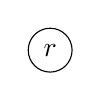
\begin{tikzpicture}
			\node [circle,draw] {\(r\)};
			\end{tikzpicture}
		\end{center}
	\end{multicols}
	\(T\) contains one node and no edges, so \(V(T) = 1\) and \(E(T) = 0\). Plug these into the proposition and we see \(1 = 0 + 1\), so the proposition holds for the base case.\\
	
	\textbf{Step}:
	\begin{multicols}{2}
		We recursively construct a new tree \(T_{new}\) by taking a root node \(r\) and pointing the left child to \(T_L\) and the right child to \(T_R\). \(T_L\) and \(T_R\) are both Non-Empty Full Binary Trees that maintain the property \(V(T) = E(T) + 1\). Here's how it looks:
		
		\columnbreak
		
		\begin{center}
			\begin{tikzpicture}[level distance=2.5cm, level 1/.style={sibling distance=3cm}]
			\node [circle,draw] {\(r\)}
			child {node [itria] {\(T_L\)}}
			child {node [itria] {\(T_R\)}};
			\end{tikzpicture}
		\end{center}
	\end{multicols}
	
	We now show that \(V(T_{new}) = E(T_{new}) + 1\). Well,
	
	\begin{center}
		\begin{tabular}{rcll}
			\(V(T_{new})\) & \(=\) & \(1 + V(T_L) + V(T_R)\) & by definition \\
			& \(=\) & \(1 + E(T_L) + 1 + E(T_R) + 1\) & by inductive hypothesis \\
			& \(=\) & \(E(T_L) + E(T_R) + 1 + 1 + 1\) & re-arranging for readability \\
			& \(=\) & \(E(T_L) + E(T_R) + 2 + 1\) & algebra \\
			& \(=\) & \(E(T_{new}) + 1\) & by definition \\
		\end{tabular}
	\end{center}
	
	The inductive step shows that by applying the recursive definition of Non-Empty Full Binary Trees the property holds true, hence \(V(T) = E(T) + 1\) by structural induction.
}

Essentially the main idea of induction is the same. We use the recursive definition, or previous element, to construct the new one, and then show the new thing maintains the proposition.

\exproof{
	A \textbf{Language} \(\mathcal{L}\) has the alphabet \(\Sigma = \{a,b,c\}\). Strings in the language are generated as follows:
	\begin{itemize}
		\item the empty string \(\epsilon \in \mathcal{L}\)
		\item \((\forall \sigma \in \mathcal{L})[ ba \sigma ab^3 \in \mathcal{L} \land cb \sigma ba^2c \in \mathcal{L} ]\)
	\end{itemize}
	
	Prove that all strings in \(\mathcal{L}\) contain an even number of \(a\)'s, \(b\)'s, and \(c\)'s.
}{
	We show the proposition via structural induction on \(\sigma\).
	
	\textbf{Base Case}:
	\begin{multicols}{2}	
		\(\sigma = \epsilon\) is the empty string:
		
		\columnbreak
		
		\begin{center}
			``''
		\end{center}
	\end{multicols}
	\(\sigma\) contains zero \(a\)'s, \(b\)'s, and \(c\)'s. Zero is even, so we are done.\\
	
	\textbf{Step}:
	\begin{multicols}{2}
		We recursively construct a new string \(\sigma_{new}\) using either of the two rules defined above, where \(\sigma \in \mathcal{L}\) is a string that maintains the proposition (ie falls in the induction hypothesis):
		
		\columnbreak
		
		\begin{enumerate}
			\item \(\sigma_{new} = ba \sigma ab^3\)
			\item \(\sigma_{new} = cb \sigma ba^2c\)
		\end{enumerate}
	\end{multicols}
	
	We now show that both new strings have even numbers of \(a\)'s, \(b\)'s, and \(c\)'s.
	
	Denote \(N(\sigma, \cdot) \equiv\) the number of input \(\cdot\) characters in \(\sigma\). The induction hypothesis tells us that \((\forall * \in \{a,b,c\})[2 \mid N(\sigma, *)]\).
	
	(1)
	
	\(N(\sigma_{new}, a) = 1 + N(\sigma, a) + 1\) is even by definition.
	
	\(N(\sigma_{new}, b) = 1 + N(\sigma, b) + 3\) is even by definition.
	
	\(N(\sigma_{new}, c) = 0 + N(\sigma, c)\) is even by definition.
	
	(2)
	
	\(N(\sigma_{new}, a) = N(\sigma, a) + 2\) is even by definition.
	
	\(N(\sigma_{new}, b) = 1 + N(\sigma, b) + 1\) is even by definition.
	
	\(N(\sigma_{new}, c) = 1 + N(\sigma, c) + 1\) is even by definition.
	
	The inductive step shows that by applying the recursive definition of \(\mathcal{L}\) the property holds true, hence every string in \(\mathcal{L}\) has an even numbers of \(a\)'s, \(b\)'s, and \(c\)'s by structural induction.
}

\subsubsection{Constructive Induction}

\index{Induction!Constructive Induction}
Our final induction technique is constructive induction. Like structural induction, there is no formal theorem for constructive induction. Instead, constructive induction utilizes the previous induction techniques.

Sometimes you will be presented a proposition with unknowns. In a linear equation, for example \(5 = 2x + 3\), you would solve for \(x\). In a proposition, for example \[(\forall n \in \N)[ 4 \mid (cn - 2)^d ]\] you would solve for \(c\) and \(d\). Constructive induction is simply doing a proof by induction to find constants that make a proposition true. In a constructive induction proof, you proceed through a regular induction proof as if your unknowns are \textit{known}. After the inductive step, you will have a handful of constraints on your unknowns. Then, you simply find actual values that satisfy your constraints.

\exproof{
	Find \(c,d \in \Z^+\) such that \((\forall n \in \N)[ 4 \mid (cn - 2)^d ]\).
}{
	We proceed via a proof by constructive weak induction.
	
	\textbf{Base}: \(n=0\), then we need \(4 \mid (c \cdot 0 - 2)^d\) which tells us that \(4 \mid (-2)^d\), and since the sign has no effect on divisibility, then \(4 \mid 2^d\) so (by UPFT) we need \(d \geq 2\).
	
	\textbf{Hypo}: Assume for some arbitrary \(n \geq 0\) that \(4 \mid (cn - 2)^d\).
	
	\textbf{Step}: Show that \(4 \mid (c(n+1) - 2)^d\).
	
	For ease, we guess that \(d = 2\). If it does not, then the induction will not work. If it does, then we were lucky!
	
	\((c(n+1)-2)^2 = (cn+c-2)(cn+c-2) = c^2n^2 + c^2n -2cn + c^2n + c^2 - 2c - 2cn - 2c + 4 = (c^2n^2 - 4cn + 4) + 2c^2n + c^2 - 4c\) and from the hypothesis \(4 \mid c^2n^2 - 4cn + 4\) so thus we need \(4 \mid 2c^2n + c^2 - 4c\). Since \(4 \mid -4c\) then we only need \(4 \mid 2c^2n + c^2\).
	
	Quite easily we can see that \(c=2\) makes the induction work. Therefore, our original guess that \(d=2\) worked!
	
	So our final proposition is \(4 \mid (2n-2)^2\) for all \(n \in \N\).
}

The above example was easy to guess without constructive induction, however this will not always be the case.

\exproof{
	Find constants \(a,b,c,d \in \R\) such that \[(\forall n \in \N)[\sum_{i=0}^{n} i^2 = an^3 + bn^2 + cn + d]\]
}{
	We proceed via a proof by constructive weak induction.
	
	\textbf{Base}: \(n=0\), then we have \(\sum_{i=0}^{0} i^2 0^2 = 0\) and \(a0^3 + b0^2 + c0 + d = d\). For the induction to work, we need the left-hand side to equal the right-hand side. Thus, \(d = 0\)
	
	\textbf{Hypo}: Assume for some arbitrary \(n \in \N\) that \(\sum_{i=0}^{n} i^2 = an^3 + bn^2 + cn\)
	
	\textbf{Step}: Show that \(\sum_{i=0}^{n+1} i^2 = a(n+1)^3 + b(n+1)^2 + c(n+1)\).
	
	We proceed like normal weak induction.
	
	\begin{align*}
	\sum_{i=0}^{n+1} i^2 &= (\sum_{i=0}^{n} i^2) + (n+1)^2 \\
	&= (an^3 + bn^2 + cn) + (n+1)^2 & \text{hypothesis}
	\end{align*}
	
	At this point, we would do some algebra and simplify to get our equation to \(= a(n+1)^3 + b(n+1)^2 + c(n+1)\). Unfortunately, we do not know what \(a,b,c\) are. This is where constructive induction comes to play -- we set the equality in question and find values of \(a,b,c\) that make the equality work!
	
	\[an^3 + bn^2 + cn + (n+1)^2 = a(n+1)^3 + b(n+1)^2 + c(n+1)\]
	
	If we expand out terms we get:
	
	LHS: \(an^3 + bn^2 + cn + n^2 + 2n + 1\)
	
	RHS: \(a(n^3 + 3n^2 + 3n + 1) + b(n^2 + 2n + 1) + c(n+1)\)
	
	Then if we match up the \(n^3\), \(n^2\), \(n^1\), and \(n^0\) terms, we get a system of equations:
	
	\begin{align*}
	an^3 &= an^3 \\
	bn^2 + n^2 &= a3n^2 + bn^2 \\
	cn + 2n &= a3n + b2n + cn \\
	1 &= a + b + c
	\end{align*}
	
	If we divide out the \(n\)'s and solve, we get:
	
	\begin{align*}
	1 &= 1 \\
	b+1 &= 3a + b  &\Rightarrow a &= \frac{1}{3} \\
	c + 2 &= 3a + 2b + c &\Rightarrow b &= \frac{2 - 3a}{2} = \frac{1}{2} \\
	1 &= a + b + c &\Rightarrow c &= 1 - a - b = \frac{1}{6}
	\end{align*}
	
	So we get \[\sum_{i=0}^{n} i^2 = \frac{1}{3}n^3 + \frac{1}{2}n^2 + \frac{1}{6}n\]
}

\begin{rem}
	The reader should verify that the above solution agrees with the known-solution
	\[\sum_{i=0}^{n} i^2 = \frac{(n)(n+1)(2n+1)}{6}\]
\end{rem}

Constructive induction is most valuable for proving upper and lower bounds on recurrences. We will discuss this in a later chapter. For now, problems like this will look as follows.

\exproof{
	Find the smallest possible \(c \in \R^+\) and \(d \in \N\) such that \(a_n \leq cd^n\) where \[a_n = \begin{cases} 2 & n = 0 \\ 4 & n=1 \\ 4a_{n-1} + 3a_{n-2} & n \geq 2 \end{cases}\]
}{
	We proceed via a proof by constructive strong induction.
	
	\textbf{Base}:
	
	\(n=0\), then we need \(a_0 \leq cd^0\) so we get \(2 \leq c\)
	
	\(n=1\), then we need \(a_1 \leq cd^1\) so we get \(4 \leq cd\)
	
	\textbf{Hypo}: Assume for all \(0 \leq i < n\) for some arbitrary \(n > 1\) that \(a_i \leq cd^i\)
	
	\textbf{Step}: Show that \(a_n \leq cd^n\).
	
	\begin{align*}
	a_n &= 4a_{n-1} + 3a_{n-2} \\
	&\leq 4cd^{n-1} + 3cd^{n-2} & \text{hypothesis}
	\end{align*}
	
	To make the induction work, we then need \(4cd^{n-1} + 3cd^{n-2} \leq cd^n\). So, we simplify this inequality and minimize our constants.
	
	\begin{align*}
	4cd^{n-1} + 3cd^{n-2} &\leq cd^n \\
	4d + 3 &\leq d^2 \\
	0 &\leq d^2 - 4d - 3
	\end{align*}
	
	Since \(d \in \N\) then we can plug in values of \(d\) into our polynomial until the inequality holds:
	\begin{center}
		\begin{tabular}{c|ccccccc}
			\(d\) & 0 & 1 & 2 & 3 & 4 & 5 & 6 \\
			\midrule
			\(d^2 - 4d - 3\) & \(-3\) & \(-6\) & \(-7\) & \(-6\) & \(-3\) & 2 & 9 \\
		\end{tabular}
	\end{center}
	
	So to minimize \(d \in \N\) and still make the inequality \(0 \leq d^2 - 4d - 3\) work we let \(d=5\).
	
	Knowing this, we go back to the base case and satisfy the constraints \(2 \leq c\) and \(4 \leq cd \Rightarrow \frac{4}{5} \leq c\). So the minimal \(c \in \R^+\) that satisfies both constraints is \(c=2\).
	
	So we get \[a_n \leq 2 \cdot 5^n\]
}

\begin{rem}
	We could have used the quadratic formula to find the exact roots, then chosen the ceiling of the positive root.
\end{rem}

Sometimes the unknown may be in a different place.

\exproof{
	Find the largest possible \(x \in \N\) such that \(a_n \leq 20n\) where \[a_n = \begin{cases} 0 & n = 0 \\ a_{\floor{n/3}} + a_{\floor{2n/5}} + xn & n > 0 \end{cases}\]
}{
	We proceed via a proof by constructive strong induction.
	
	\textbf{Base}:
	
	\(n=0\), then we have \(a_0 = 0 \leq 0 = 20 \cdot 0\). We learn nothing from the base case.
	
	\textbf{Hypo}: Assume for all \(0 \leq i < n\) for some arbitrary \(n > 0\) that \(a_i \leq 20i\)
	
	\textbf{Step}: Show that \(a_n \leq 20n\). During the process, we will find a value for \(x\).
	
	\begin{align*}
	a_n &= a_{\floor{n/3}} + a_{\floor{2n/5}} + xn \\
	&\leq 20\floor{n/3} + 20\floor{2n/5} + xn & \text{hypothesis} \\
	&\leq 20\frac{n}{3} + 20\frac{2n}{5} + xn & \text{floor defn.} \\
	&\leq 20n
	\end{align*}
	
	To make the induction work, we simplify the inequality:
	
	\begin{align*}
	20\frac{n}{3} + 20\frac{2n}{5} + xn &\leq 20n \\
	\frac{20}{3} + \frac{40}{5} + x &\leq 20 \\
	20 + 3 \cdot 8 + 3x &\leq 60 \\
	3x &\leq 60 - 20 - 24 \\
	x &\leq \frac{16}{3} = 5 + \frac{1}{3}
	\end{align*}
	
	Since \(x \in \N\) the largest value of \(x\) that works is \(5\). So we get \[x = 5\]
}

\subsubsection{Induction Templates}

Here are some templates we use for induction proofs. These should be used as a starting point until you fully understand what is going on. Some professors may do induction proofs differently -- follow their style.

\textbf{Weak Induction}

\textit{Style 1}
\begin{proof}
	Let \(P(n)\) be the proposition \textit{insert statement here}. We proceed via W.M.I.\ on \(n\).
	
	\textbf{Base}: Prove \(P(\text{\textit{lowest base case index}})\)
	
	\textit{insert math here that shows the proposition is true for the lowest base case}
	
	\textbf{Hypo}: Assume \(P(n)\) is true for arbitrary \(n \geq \text{\textit{lowest base case index}}\), i.e.: \textit{plug \(n\) into the proposition}
	
	\textbf{Step}: Show \(P(n) \Rightarrow P(n+1)\), i.e.: \textit{plug \(n+1\) into the proposition}
	
	\textit{insert math here, making sure you \textbf{use the IH}}
	
	The IS is true, hence by the P.M.I.\ \textit{insert full proposition} is true.
\end{proof}

\textit{Style 2}
\begin{proof}
	Let \(P(n)\) be the proposition \textit{insert statement here}. We proceed via W.M.I.\ on \(n\).
	
	\textbf{Base}: Prove \(P(\text{\textit{lowest base case index}})\)
	
	\textit{insert math here that shows the proposition is true for the lowest base case}
	
	\textbf{Hypo}: Assume \(P(n-1)\) is true for arbitrary \(n > \text{\textit{lowest base case index}}\), i.e.: \textit{plug \(n-1\) into the proposition}
	
	\textbf{Step}: Show \(P(n-1) \Rightarrow P(n)\), i.e.: \textit{plug \(n\) into the proposition}
	
	\textit{insert math here, making sure you \textbf{use the IH}}
	
	The IS is true, hence by the P.M.I.\ \textit{insert full proposition} is true.
\end{proof}

\textbf{Strong Induction}

\begin{proof}
	Let \(P(n)\) be the proposition \textit{insert statement here}. We proceed via S.M.I.\ on \(n\).
	
	\textbf{Base}: Prove \(P(k)\) for all \(k\) base case indices
	
	\textit{insert math here that shows the proposition is true for every base case}
	
	\textbf{Hypo}: Assume \(P(i)\) is true for all \(\text{\textit{lowest base index}} \leq i \leq n-1\) for arbitrary \(n-1 \geq \text{\textit{highest base case index}}\), i.e.: \textit{plug \(i\) into the proposition}
	
	\textbf{Step}: Show \(P(n)\), i.e.: \textit{plug \(n\) into the proposition}
	
	\textit{insert math here, making sure you \textbf{use the IH}}
	
	The IS is true, hence by the P.M.I.\ \textit{insert full proposition} is true.
\end{proof}

\textbf{Structural Induction}

\begin{proof}
	We show \textit{insert statement here} via Structural Induction on \textit{the variable that represents the structure}.
	
	\textbf{Base}: \textit{show the statement holds for every base case laid out in the recursively-defined structure}
	
	\textit{insert math here}
	
	\textbf{Hypo}: \textit{okay to omit}
	
	\textbf{Step}: We recursively construct a new \textit{object} by \textit{precisely follow the recursive definition}. The \textit{recursive} part(s) of the new object fall in the inductive hypothesis, so satisfy the property \textit{plug those recursive parts into the statement}. \textit{show a picture of the new structure}. We now show the property holds for our new structure.
	
	\textit{insert math here, making sure you \textbf{use the IH}}
	
	The IS is true, hence by Structural Induction \textit{insert full proposition} is true.
\end{proof}

\textbf{Constructive Induction}

Just follow the previous techniques. At the end of the step, usually you will be solving some form of algebraic system.

% todo -- loop invariance? maybe save for asymp anal?

\subsection{Combination of Techniques}

We can combine our previously-defined proof techniques to accomplish any goal we want.

\begin{defn}[Proof by Cases]
	A more general proof technique where you break a statement into multiple sub-statements, and prove each sub-statement individually. The sub-statements \textbf{must} fully cover the original statement (there cannot be anything missing)
\end{defn}

\exsol{
	Explain, for the statement \((\forall x \in \Z)[2 \mid x^2 + x]\), why the following proof is invalid.
	
	\begin{proof}[boxrule=0pt]
		When \(x\) is even then \(\exists k \in \Z\) such that \(x = 2k\), and thus \(x^2 + x = (2k)^2 + 2k = 4k^2 + 2k = 2(2k^2 + k) = 2q\) where \(q = 2k^2 + k \in \Z\) by closure of integers under addition and multiplication. So \(x^2 + x\) is divisible by 2 by definition
	\end{proof}
}{
	It is invalid because the proof does not fully cover all possibilities of the statement. The proof covers all even integers, however odd integers are nowhere found in the proof. Clearly \(\Z \neq \Z^{\text{even}}\).
	
	This proof should have been a proof by cases. One case is the proof already given, and the other case should be when \(x\) is odd.
}

\exproof{
	Finish the previous proof.
}{
	(continued)
	
	Case 2: \(x\) is odd, then \(\exists l \in \Z\) such that \(x = 2l + 1\), then \(x^2 + x = (2l+1)^2 + 2l+1 = 4l^2 + 4l + 1 + 2l + 1 = 4l^2 + 6l + 2 = 2(2l^2+3l+1) = 2r\) where \(r = 2l^2+3l+1 \in \Z\) by closure of integers under addition and multiplication. So \(x^2 + x\) is divisible by 2 by definition
	
	Both cases cover the entirety of the integers by parity, thus the statement holds for all integers
}

\begin{rem}
	Both cases in the previous proof were direct proofs, however in other examples there could be cases that are proven indirectly. The previous proof used two cases, however there could be examples using more (e.g.\ if you want to prove \((\forall a \in \Z)[7 \mid a^2 \Rightarrow 7 \mid a]\)).
\end{rem}

\section{Summary}

\begin{itemize}
	\item There are many definitions and concepts in number theory.
	\item There are many proof techniques in number theory.
	\item To be good at proofs, you must internalize all definitions, think outside the box, and practice a lot.
\end{itemize}

\section{Practice}

\begin{enumerate}
	\item Re-write the following sum as a summation: \[1-4+7-10+13-16+19-22+ \cdots \pm (3n-2)\]
	\item Re-write the following product as a product: \[n^{1/2} \times (2n)^{1/4} \times (3n)^{1/6} \times (4n)^{1/8} \times \cdots \]
	\item Calculate \(\log_2 3 \times \log_3 4 \times \cdots \times \log_{31} 32\) without a calculator.
	\item Show that \(\floor{x} + \floor{y} \leq \floor{x+y} \leq \floor{x} + \floor{y} + 1\) for all \(x,y \in \R\).
	\item Show that \(\floor{x} = x \Leftrightarrow x \in \Z\).
	\item Explain the difference between \(\equiv\) (congruence) and \(\%\) (remainder).
	\item Show that \((\forall m,n \in \Z^{\neq 0})[(n \mid m \land m \mid n) \Rightarrow m = \pm n]\).
	\item Come up with a rule for \(\Mod{4}\) and \(\Mod{11}\).
	\item Fill in the following number-base translation table:
	
	\begin{tabular}{c|c|c|c}
		Base 2 & Base 8 & Base 16 & Base 10 \\
		\midrule
		10110 & & & \\
		\midrule
		& 703 & & \\
		\midrule
		& & 0xDAB & \\
		\midrule
		& & & 1000
	\end{tabular}
	
	\item Prove there is no smallest integer.
	\item Prove \(7 \mid a^2 \Rightarrow 7 \mid a\) for any \(a \in \Z\).
	\item Prove \(2 \mid a^3 \Rightarrow 2 \mid a\) for any \(a \in \Z\). Then prove that \(\sqrt[3]{2} \not\in \Q\) by the Euclidean Argument and by UPFT.
	\item Generalize the lemmas used in the root-irrationality proofs -- namely, prove that for any prime \(p\), integer \(a\), and integer \(n > 1\), \(p \mid a^n \Rightarrow p \mid a\). Then, prove the general claim that \(\sqrt[n]{p} \not\in \Q\) by the Euclidean Argument and by UPFT.
	
	\item Show that \(2 \mid n(n+1)\) using a direct proof and using weak induction.
	\item Show that for any \(n \times n\) matrix \(A\) with \(n > 1\) that \[\sum_{i=2}^{n} \sum_{j=1}^{i-1} A_{ij} = \sum_{j=1}^{n-1} \sum_{i=j+1}^{n} A_{ij}\] where \(A_{ij}\) is the value of \(A\) in the \(i\)-th row and \(j\)-th column.
	
	\item Prove that \(\sqrt[n]{n} < 2 - \frac{1}{n}\) for all \(n \geq 2\).
	\item Prove \(\forall x \neq 0,\ \forall n \in \N^{>1}\) that \(x^2 \mid ((x+1)^n - nx - 1)\)
	\item Prove the coin problem in Example \ref{2coin-problem} using weak induction. % todo fix this example, it shows 3.3.2 but that's wrong i think
	\item Prove \(\big(\bigwedge_{i=1}^{n-1} (p_i \Rightarrow p_{i+1})\big) \Rightarrow \big( (\bigwedge_{i=1}^{n-1} p_i) \Rightarrow p_n \big)\) for all \(n > 1\)
	
	\item Prove that \((\forall n \in \N)[s_n \equiv 0 \Mod{2}]\) where \[s_n = \begin{cases} 2, & n = 0 \\ 4, & n = 1 \\ 3s_{n-1} + s_{n-2},& n \geq 2 \end{cases}\]
	\item Solve the quadratic equation \(x^2 - x - 1 = 0\) -- name the larger root \(\phi\) and the smaller root \(\psi\). Then, justify why \(\phi^2 = \phi + 1\) and \(\psi^2 = \psi + 1\). Finally, use these to show that \(f_n = \frac{\sqrt{5}}{5}(\phi^n - \psi^n)\) where \[f_n = \begin{cases} 0 & n=0 \\ 1 & n=1 \\ f_{n-1} + f_{n-2} & n \geq 2 \end{cases}\]
	\item Let \[l_n = \begin{cases} 2 & n=0 \\ 1 & n=1 \\ l_{n-1} + l_{n-2} & n \geq 2 \end{cases}\]
	Show that \(l_n = \phi^n + \psi^n\)
	
	\item Let \(S \subset \Z^2\) be defined recursively as:
	\begin{itemize}
		\item\((0,0) \in S\)
		\item \((\forall (x,y) \in S)[(x,y+1) \in S \land (x+1,y+1) \in S \land (x+2,y+1) \in S]\)
	\end{itemize}
	Prove that \((\forall (x,y) \in T)[x \leq 2y]\)
	\item Show that every Non-Empty Full Binary Tree \(T\) satisfies
	\begin{enumerate}
		\item \(l(T) = I(T) + 1\)
		\item \(EXT(T) = INT(T) + N(T) - 1\)
	\end{enumerate}
	where
	\begin{itemize}
		\item \(l(T) = \) the number of leaf nodes (nodes without children) in \(T\)
		\item \(I(T) = \) the number of internal nodes (nodes with children) in \(T\)
		\item \(EXT(T) = \) the sum of all external path lengths in \(T\). An external path is a path from the root node to any leaf node, and the length is the number of edges in that path
		\item \(INT(T) = \) the sum of all internal path lengths in \(T\). An internal path is a path from the root node to any internal node
	\end{itemize}
	\item Show that the number of nodes in a perfect \(k\)-ary tree is \(\sum_{i=0}^{h} k^i\) (which, by the geometric series \(= \frac{k^{h+1}-1}{k-1}\)) where \(h =\) the height of the tree, and \(k\) is the branching factor of the tree. Define height as the maximal external path length. Define a perfect \(k\)-ary tree as follows:
	\begin{itemize}
		\item \(h = 0\): a single root node
		\item \(h > 0\): a root node with exactly \(k\) children (each of which is a perfect \(k\)-ary tree of height \(h-1\)
	\end{itemize}
	
	\item Prove that \((\forall n \in \N^{\geq n_0})[2^n > \frac{1}{24}(n^4 - 6n^3 + 23n^2 - 18n + 24)]\), then use your proof to find \(n_0 \in \N\)
	\item Prove \((\exists a,b \in \N)(\forall n \in \N)[7 \mid a^n + b]\)
	\item Find constants \(a,b,c,d,e \in \R\) such that \[(\forall n \in \N)[\sum_{i=0}^{n} i^3 = an^4 + bn^3 + cn^2 + dn + e]\]
	\item Prove that \(t_n \leq n \log_b n\) where \[t_n = \begin{cases} 0, & n = 0 \\ 2t_{\floor{\frac{n}{2}}} + n - 1, & n > 0 \end{cases}\] \textit{you will need to select a base \(b \in \Z^+\) during the step that makes the induction easy}
	\item Find the lower bound for the amount of dollars we can make using strictly 5 and 6 dollar bills. Do this with constructive induction. Verify your result is correct by proving it with both weak and strong induction. % >= 20
	\item Repeat the previous problem with strictly 3, 7, and 15 dollar bills.
\end{enumerate}

%\section{Solutions}
%
%\begin{enumerate}
%	\item Bottom Text
%	\item Proof follows:\\
%	\begin{proof}
%		We proceed via weak mathematical induction on \(n\)
%	\end{proof}
%	\item Bottom Text
%\end{enumerate}
\end{document}
